\documentclass[11pt]{article}
\usepackage[margin=.73in]{geometry}
\usepackage{lmodern,amsmath,amssymb,booktabs,graphicx,microtype,fancyhdr,xurl,hyperref,array}
\hypersetup{colorlinks=true,urlcolor=blue,linkcolor=black,pdftitle={HPS GPR v6.4.2: 2016 and combined signal-MC extraction}}
\pagestyle{fancy}\fancyhf{}\lhead{HPS GPR: 2016 and combined signal-MC extraction}\rhead{v6.4.2}\cfoot{\thepage}
\setlength{\headheight}{14pt}\setlength{\parindent}{0pt}\setlength{\parskip}{6pt}\setlength{\emergencystretch}{2em}
\newcommand{\Ah}{\widehat A}\newcommand{\sh}{\widehat\sigma}
\begin{document}
{\LARGE\bfseries The 2016 signal shape\par and its effect on the combined analysis}\par
{\large HPS Gaussian-process background analysis}\par
25 September 2026\hfill Version 6.4.2

\textbf{The result.} The supplied smeared 2016 signal MC has a reconstructed core slightly below the generated mass. Its displacement is 0.08--1.02 MeV over the adopted 40--175 MeV domain, and its tails are measurably non-Gaussian. The new extraction uses the full empirical signal shape, interpolated between neighboring MC masses, with the fit and GP-training exclusion centered on that shape's fitted core.

For 2016 the interval is $-3.5\le u\le+3.5$; for 2021 the latest $-4\le u\le+3$ interval is retained. Here $u=(m_{\rm rec}-c)/s$, with each year's MC core center $c$ and core width $s$. The 2015 Gaussian remains unchanged.

\textbf{What changes in the observations?} The strongest 2016 MC-template region is at a generated mass of 91 MeV, followed by a disjoint fitted region at 69 MeV. The 91 MeV fit gives $\Ah=20{,}201\pm5{,}699$ full selected MC events and a conditional 90\% profile-limit of 27,505 events. Its local asymptotic probability is $0.000196$, but the fixed-source background check has 3 exceedances in 1,000 toys. The difference is material: the background source produces a positive mean fitted signal in this region. The report shows both probability descriptions.

The combined MC-template analysis has its smallest local asymptotic probability at 68 MeV, $p_0=0.00248$. Over 60--175 MeV, replacing the 2016 Gaussian in the existing 2021-MC combination changes the conditional profile upper limit by a median $+1.26\%$, with a range from $-6.39\%$ to $+12.49\%$. These changes include both the signal shape and the fit/training window.

\begin{center}\small\begin{tabular}{>{\raggedright\arraybackslash}p{1.30in}>{\raggedright\arraybackslash}p{1.12in}>{\raggedright\arraybackslash}p{1.12in}>{\raggedright\arraybackslash}p{1.75in}}\toprule
Combined comparison & 2015 & 2016 & 2021\\\midrule
All Gaussian & Gaussian & Gaussian & Established shifted Gaussian\\
2021 MC only & Gaussian & Gaussian & Shifted neighbor MC, $[-4,+3]u$\\
2016 + 2021 MC & Gaussian & Shifted neighbor MC, $\pm3.5u$ & Shifted neighbor MC, $[-4,+3]u$\\\bottomrule
\end{tabular}\end{center}

\textbf{Reading guide.} The first part explains the native histograms, their centers, overlays and interpolation. The extraction section defines the windows, likelihood and normalization before showing the 2016 scan, two fitted excess regions, and the three combined comparisons. Fixed-source toy checks distinguish the local probability and discrete fixed-source rank endpoints from the continuous profile curves. The catalogue shows every supplied 2016 histogram. Appendix A (page~\pageref{sec:windowappendix}) compares a narrower $\pm2u$ window for 2016; the main-body analysis remains at $\pm3.5u$.

The observations are the archived full 2015 and 2016 spectra and the archived 2021 10\% spectrum. All probabilities are local and conditional on the specified models. The numerical comparisons do not establish a scan-wide discovery probability or a detector-qualified physical exclusion.
% Signal-MC shape material; figures are regenerated from the pinned v6.4 inputs.
% The root report supplies the preamble and the running figure counter.
\clearpage\section*{2016 signal MC: where does the reconstructed core lie?}

\textbf{The result.} The supplied 2016 signal histograms have a small downward core displacement over 40--175 MeV: the fitted center is 0.08--1.02 MeV below the generated mass. The sign agrees with the saved 2021 samples, but the displacement is smaller. The selected distributions also have measurable non-Gaussian tails. These observations motivate using each year's own MC shape and core location in the extraction that follows.

\textbf{Inputs.} The 29 ROOT files contain 3,770,135 selected entries at generated masses from 30 to 175 MeV, in nominal 5 MeV steps; the 150 MeV sample is missing. The analyzed histogram is \texttt{h\_MinvScSm\_GeneralLargeBins\_Final\_1}. According to the supplied sample description, it contains prompt target-constrained signal with FEE momentum scaling and smearing already applied. No additional smearing is applied here. The unsmeared histogram is inventoried but is not used to determine the template.

\begin{center}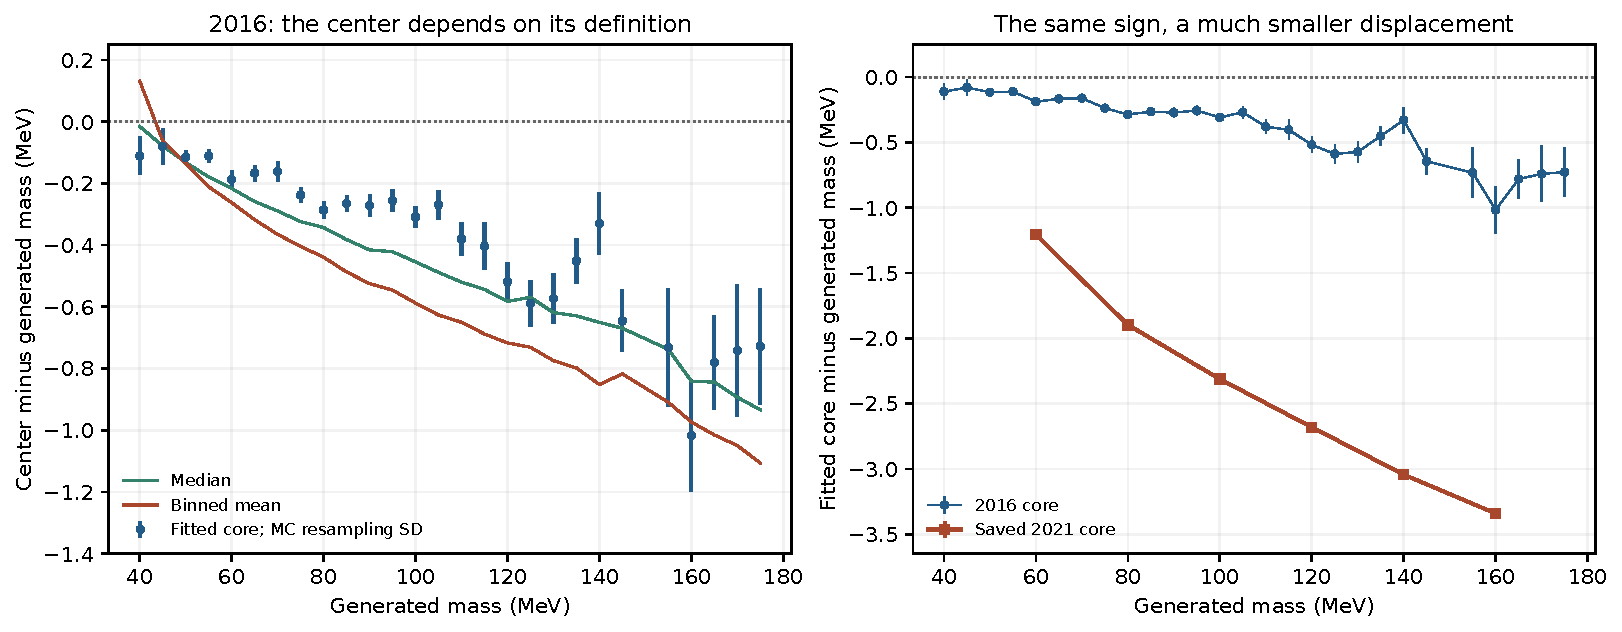
\includegraphics[width=\linewidth,height=3.3in,keepaspectratio]{../figures/shape_centers_and_2021.pdf}\end{center}
{\small\refstepcounter{figure}\textbf{Figure \thefigure. How to read the figure.} Left: the fitted core, median and binned mean answer different location questions because the distributions have tails. Right: the 2016 core locations are compared with the earlier v6.1 2021 results using the same local-core convention. The extraction later uses the separate latest v16 TC bank. Bars are the standard deviation over MC bin-resampling fits: 64 replicas for 2016 and 32 for 2021. They describe finite-MC variation, not detector calibration uncertainty. Reconstruction and selection equivalence between the two sets of samples has not been established.}\par\medskip

\begin{center}\small\begin{tabular}{rrrr}\toprule
Generated mass [MeV] & 2016 core [MeV] & Shift [MeV] & MC SD [MeV]\\\midrule
60 & 59.812 & $-0.188$ & 0.028\\
100 & 99.691 & $-0.309$ & 0.034\\
160 & 158.983 & $-1.017$ & 0.181\\
\bottomrule\end{tabular}\end{center}

The fitted core locates the main peak. The median divides the full selected probability in half. The mean includes the entire tail and can move when a small amount of probability lies far from the peak. The core is the location used to align templates; the mean and median remain useful independent descriptions. The 30 and 35 MeV samples require separate treatment below, so the primary template domain begins at 40 MeV.

\clearpage\section*{How are the core center and width defined?}

The locator follows the convention used for the signal-MC comparisons in v6.3.6. It finds a smoothed mode within three reference analysis widths of the generated mass, then fits the unsmoothed bins within 1.5 reference widths of that mode. The model is a bin-integrated Gaussian plus a nonnegative affine pedestal, fitted by Poisson deviance. The pedestal describes the broad signal shoulders locally; it is not a collision-background component.

\begin{center}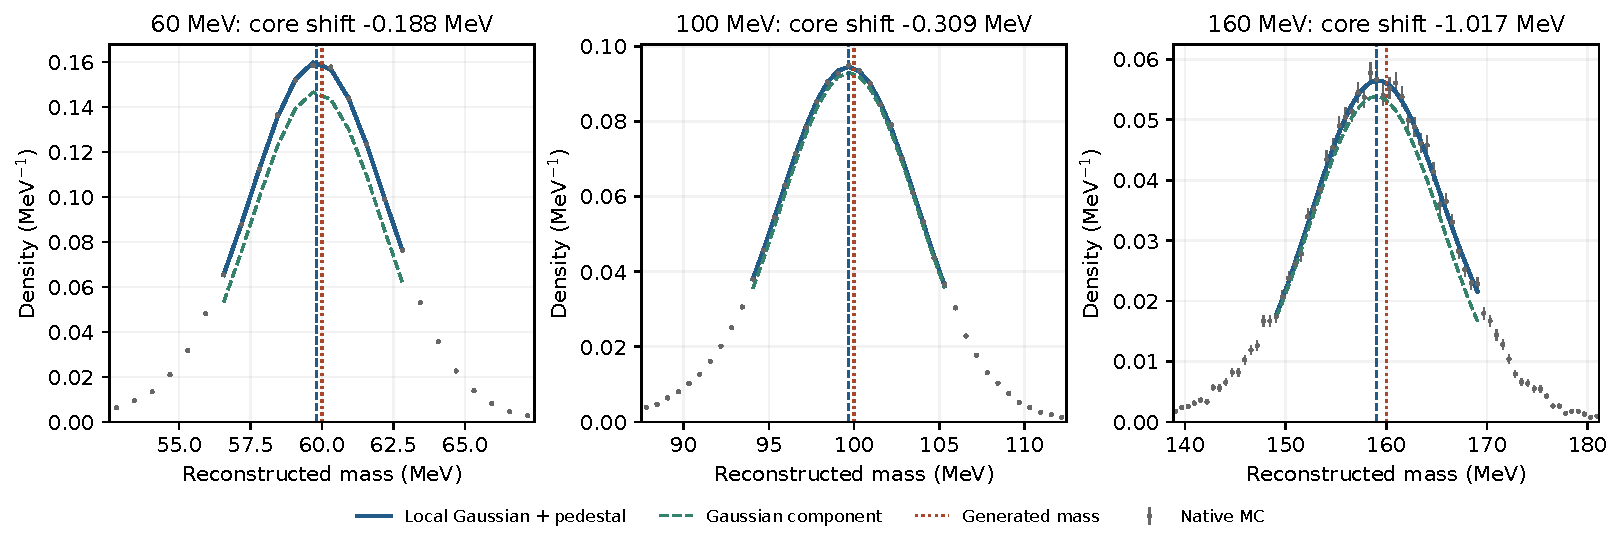
\includegraphics[width=\linewidth,height=2.0in,keepaspectratio]{../figures/shape_core_fit_examples.pdf}\end{center}
{\small\refstepcounter{figure}\textbf{Figure \thefigure. How to read the figure.} Points are the native 0.625 MeV bins, with square-root-count bars. Blue: the local Gaussian plus pedestal, drawn only across its fitted bins. Green: its Gaussian component. The red vertical line is the generated mass; the blue dashed line is the fitted core. Integrating the model over each bin avoids defining the center by the tallest bin alone.}\par\medskip

\begin{center}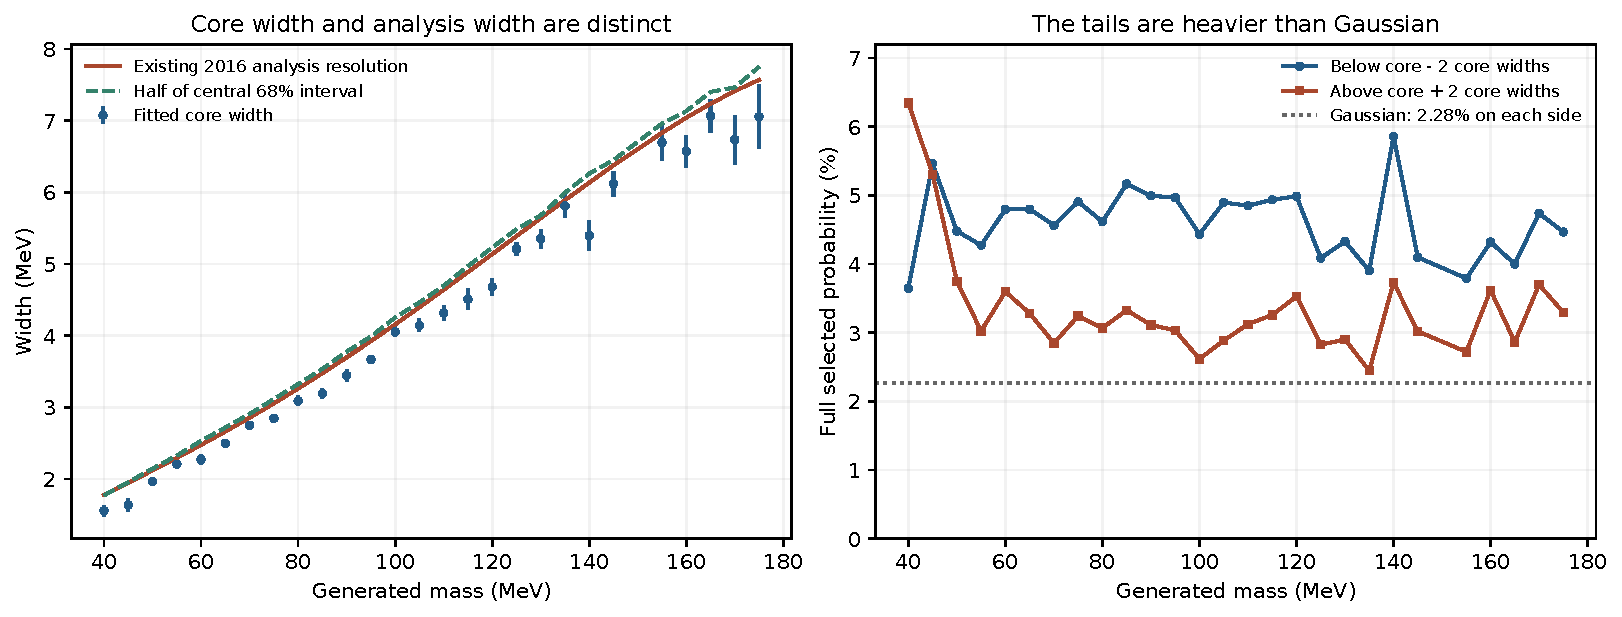
\includegraphics[width=\linewidth,height=2.05in,keepaspectratio]{../figures/shape_widths_and_tails.pdf}\end{center}
{\small\refstepcounter{figure}\textbf{Figure \thefigure. How to read the figure.} Left: fitted core width, existing 2016 analysis-resolution curve, and half the central 68\% probability interval. These are distinct width definitions. Right: full selected probability below and above two fitted core widths. A Gaussian has 2.28\% on each side. Core-width bars are MC resampling standard deviations.}\par\medskip

The core width grows from 1.56 MeV at 40 MeV to 7.06 MeV at 175 MeV and is 0.84--0.99 times the reference analysis width. Between 89.2\% and 93.7\% of selected probability is within two core widths, compared with 95.45\% for a Gaussian. The reference-width curve helps define the locator; the new MC extraction instead uses the interpolated fitted core width to define its window.

All 1,728 resampling fits in the primary domain pass the locator checks. A separate definition test varies the fitting range and removes the pedestal. The largest center change at 60, 100 and 160 MeV is 0.044, 0.084 and 0.396 MeV. This spread is reported separately from the MC error: it shows that a precise statistical center can still depend on the local-fit definition.

\clearpage\section*{Overlay the distributions while retaining their tails}

\begin{center}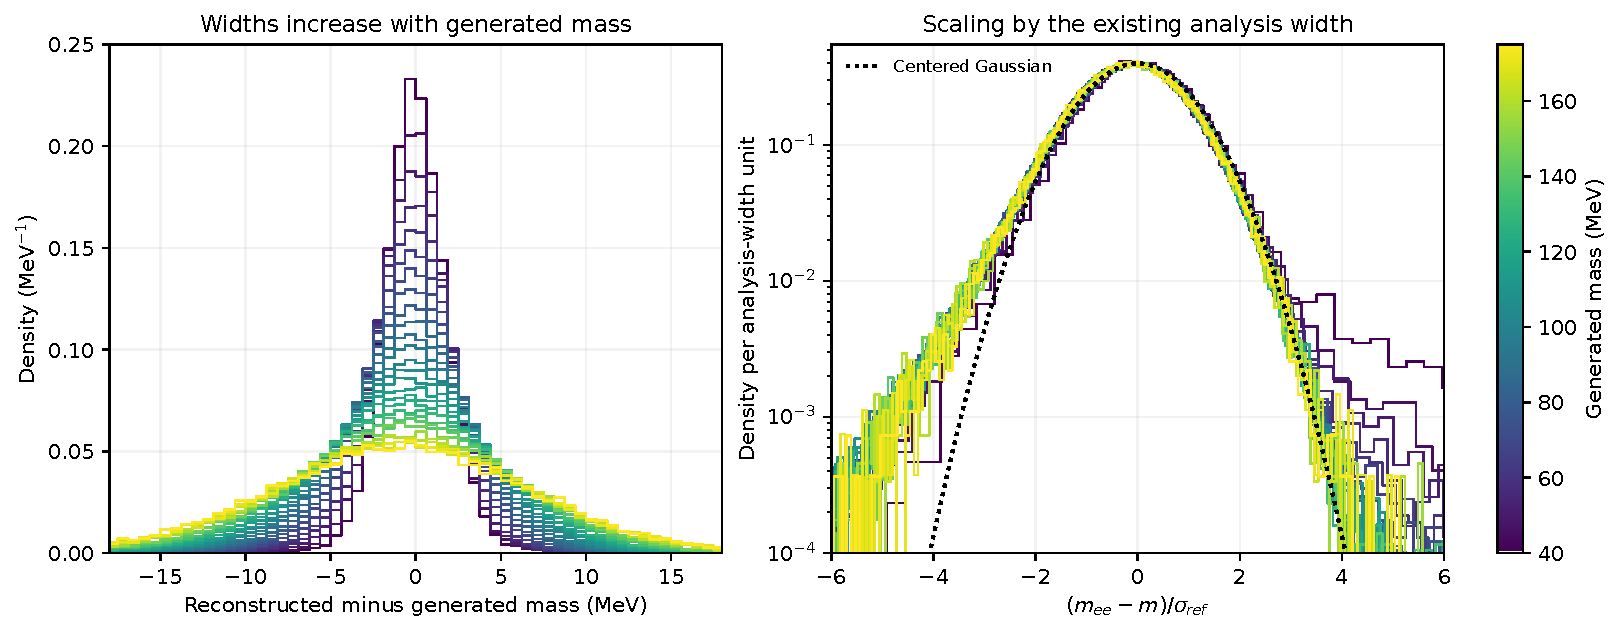
\includegraphics[width=\linewidth,height=3.05in,keepaspectratio]{../figures/shape_generated_aligned_overlays.pdf}\end{center}
{\small\refstepcounter{figure}\textbf{Figure \thefigure. How to read the figure.} Every colored curve is one native 2016 histogram divided by its own full selected count. Left: subtracting the generated mass leaves the growth in width visible. Right: scaling by the existing analysis width brings the curves closer together. The dotted Gaussian is centered at the generated mass. The logarithmic scale reveals tail differences. Neither panel renormalizes the displayed mass range.}\par\medskip

\begin{center}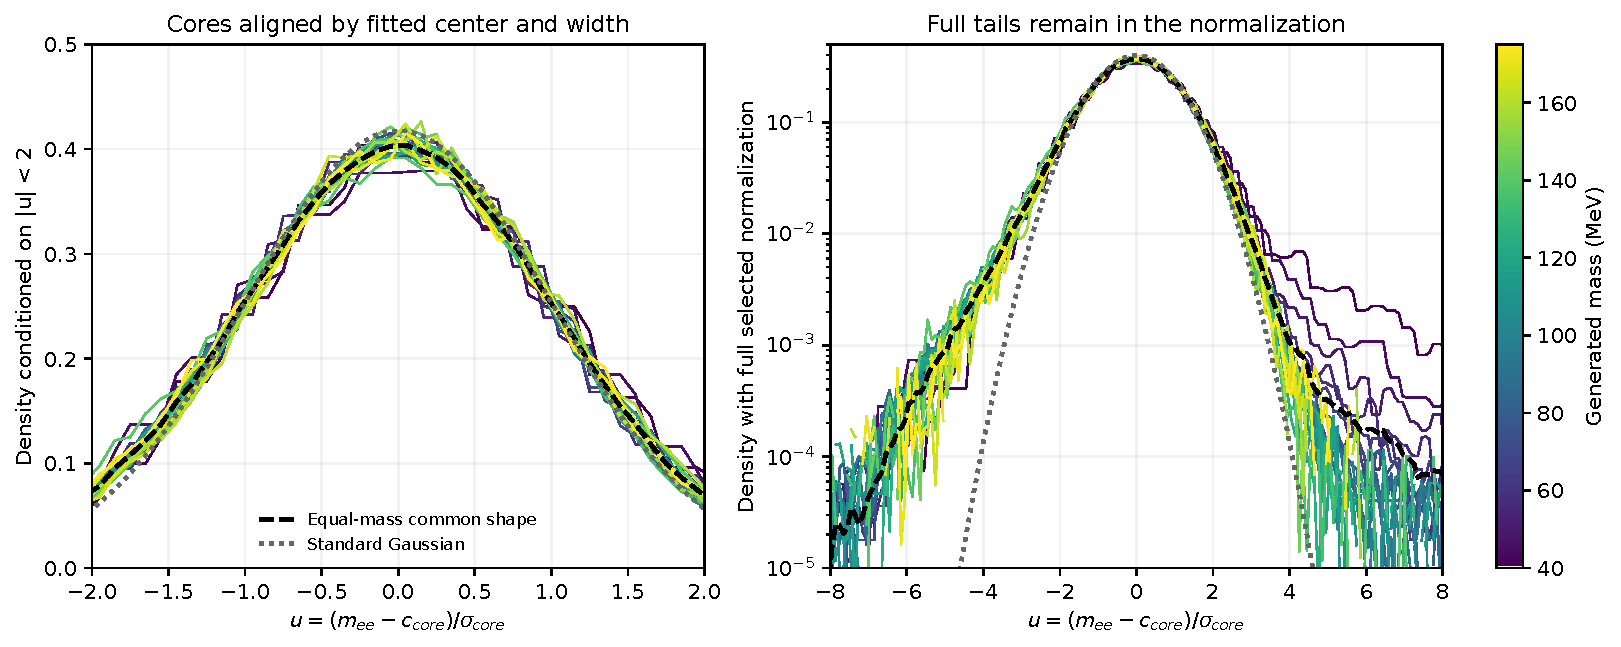
\includegraphics[width=\linewidth,height=3.05in,keepaspectratio]{../figures/shape_core_aligned_overlays.pdf}\end{center}
{\small\refstepcounter{figure}\textbf{Figure \thefigure. How to read the figure.} Here $u=(m_{\rm rec}-c)/s$, where $c$ and $s$ are each histogram's fitted core center and width. Left: each distribution is conditioned on $|u|<2$ to compare central shapes. Right: its full selected normalization is restored. The black dashed curve is an equal-mass average of the 27 aligned empirical distributions; the gray dotted curve is a standard Gaussian with the corresponding normalization.}\par\medskip

\textbf{Answer.} Alignment produces similar central shapes, but it does not make the complete distributions identical. Conditioning on the core hides differences in the amount of signal outside it. The full-distribution panel shows why a common core description can be useful while a mass-dependent MC template is still preferable for the selected signal yield.

\clearpage\section*{Use separate empirical centers for 2016 and 2021}

\textbf{The 2021 displacement should not be transferred to 2016.} At generated masses of 60, 100 and 160 MeV, the saved 2021 core shifts are $-1.208$, $-2.312$ and $-3.342$ MeV. The corresponding 2016 shifts are $-0.188$, $-0.309$ and $-1.017$ MeV. Both the locations and the tail probabilities differ.

\begin{center}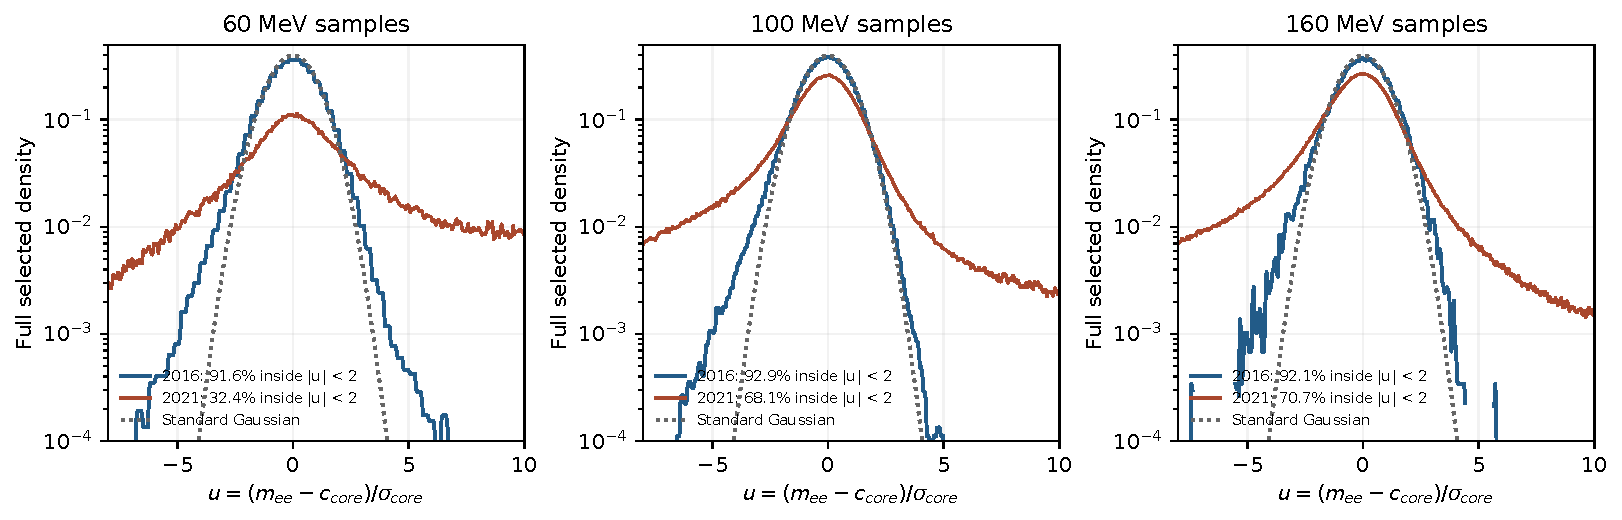
\includegraphics[width=\linewidth,height=3.25in,keepaspectratio]{../figures/shape_cross_year_shapes.pdf}\end{center}
{\small\refstepcounter{figure}\textbf{Figure \thefigure. How to read the figure.} Each year is aligned by its own fitted core center and width. Curves retain full selected normalization, including the saved 2021 overflow normalization. The percentages give the probability within $|u|<2$. The 2016 samples are more concentrated around their cores. This compares the supplied samples; it does not identify whether reconstruction, selection, calibration or another difference causes the change.}\par\medskip

For orientation, an equal-weight affine fit to the 2016 core shifts gives
\[
 c(m)=m-0.363673-0.563179\frac{m-100}{100},
 \qquad 40\le m\le175\ \mathrm{MeV},
\]
with all masses in MeV. Leaving out each mass in turn gives an RMS prediction error of 0.103 MeV and a largest absolute error of 0.351 MeV. This is a compact description of the trend. The extraction uses the empirical centers and their local interpolation instead, so it preserves the measured mass dependence without imposing this smooth law.

\textbf{The coordinate used by the MC method.} At a tested generated mass $m$, let $c_y(m)$ and $s_y(m)$ be the interpolated core center and width for year $y$. Then
\[
 u_y=\frac{m_{\rm rec}-c_y(m)}{s_y(m)}.
\]
The adopted 2016 fit and GP-training exclusion use $-3.5\le u_{2016}\le+3.5$. The 2021 method retains $-4\le u_{2021}\le+3$. Thus each window follows its own reconstructed MC core. The tested mass remains the generated signal mass, and is the horizontal coordinate of the limit and local-probability scans.

These shifts describe selected MC after its stated scaling and smearing. They do not establish a data mass-scale correction or identify the physical cause of the displacement. The saved 2021 signal-MC reference is the same input used for the introductory shape comparisons in v6.3.6.

\clearpage\section*{Why use the neighboring MC templates?}

\textbf{The comparison.} A Gaussian at the measured core, a common aligned empirical shape, and interpolation of the nearby samples are compared with the native histograms. For the common shape and neighbor tests, the tested histogram is omitted when constructing the approximation. The neighbor method must predict its center and width as well as its standardized shape.

\begin{center}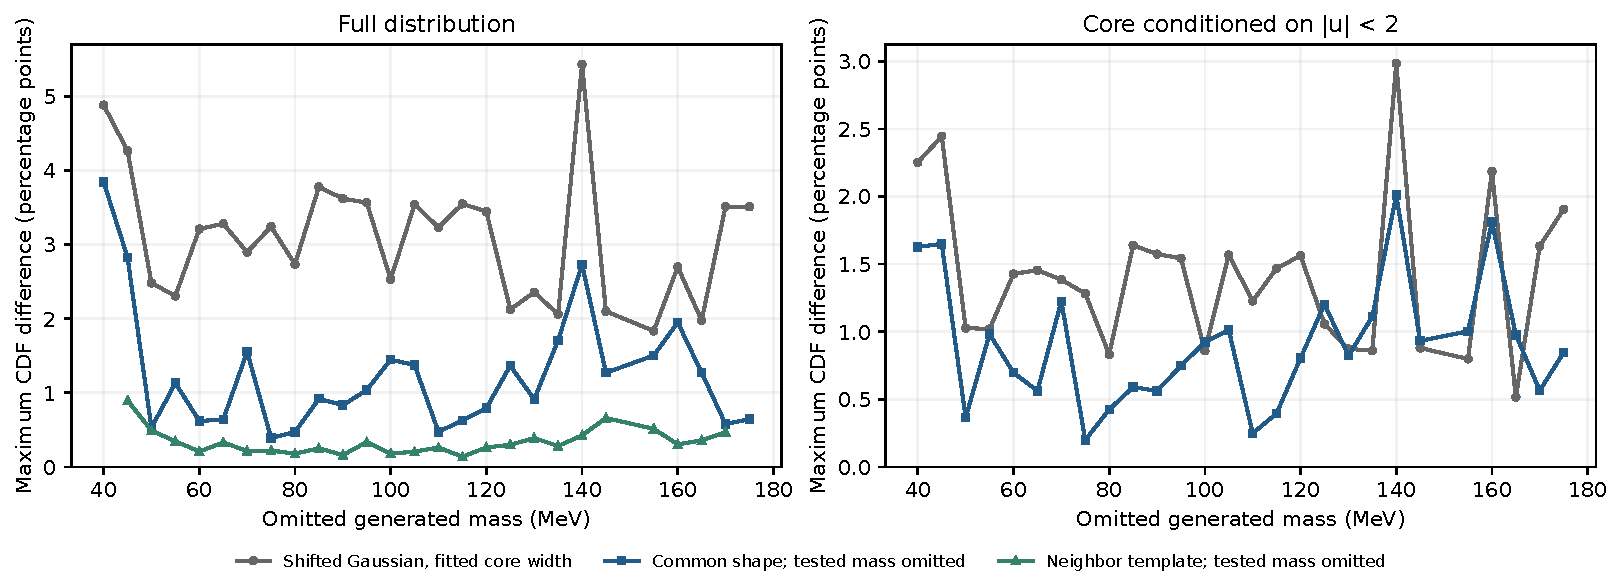
\includegraphics[width=\linewidth,height=3.2in,keepaspectratio]{../figures/shape_shape_holdout.pdf}\end{center}
{\small\refstepcounter{figure}\textbf{Figure \thefigure. How to read the figure.} The vertical axis is the largest absolute cumulative-probability difference, in percentage points: at native bin boundaries for the full distribution, and on a common standardized grid for the core. A value of one means that the integrated probabilities differ by one percentage point at some bin boundary. It is a shape discrepancy, not a $p$-value. The neighbor curve uses linear interpolation of both core center and width, as in the new extraction. Core-only comparisons condition on $|u|<2$ and use the measured center and width.}\par\medskip

\begin{center}\small\begin{tabular}{lrrr}\toprule
Full-distribution approximation & Median difference & Range & Tests\\\midrule
Gaussian at measured core & 3.23 pp & 1.83--5.43 pp & 27\\
Gaussian at full mean and RMS & 2.05 pp & 1.54--8.10 pp & 27\\
Common shape, tested mass omitted & 1.04 pp & 0.39--3.84 pp & 27\\
Neighbor template, tested mass omitted & 0.30 pp & 0.14--0.90 pp & 25\\
\bottomrule\end{tabular}\end{center}

\textbf{The adopted template.} At a simulated mass, use the native histogram. Between two simulated masses, linearly interpolate their core centers and core widths, align both histograms in $u$, and mix their cumulative distributions with the same mass interpolation weights. Taking differences of the resulting cumulative probabilities gives the probability in every requested analysis bin. The full selected normalization is retained throughout; fitting a finite window does not redefine the total signal yield.

The 150 MeV shape is interpolated between 145 and 155 MeV, because no 150 MeV input exists. The 40 and 175 MeV endpoints have no two-sided omitted-mass test. The older v6.4 shape study interpolated the logarithm of the width; this revision uses the linear-width convention shared with the latest 2021 neighbor method. The plotted neighbor checks have been recalculated for that convention. Linear interpolation has a slightly larger median discrepancy (0.30 rather than 0.24 percentage points); it is adopted for a consistent convention across years, not as an improvement over logarithmic-width interpolation.

The neighbor template gives the closest agreement in these omitted-mass shape checks. Finite-MC variation contributes to every discrepancy. These checks support the template choice, but they do not by themselves calibrate background absorption, limit coverage, or an uncertainty band for arbitrary intermediate masses. Those are different questions from how accurately one selected MC distribution predicts another.

\clearpage\section*{The 2016 window and the low-mass exceptions}

\begin{center}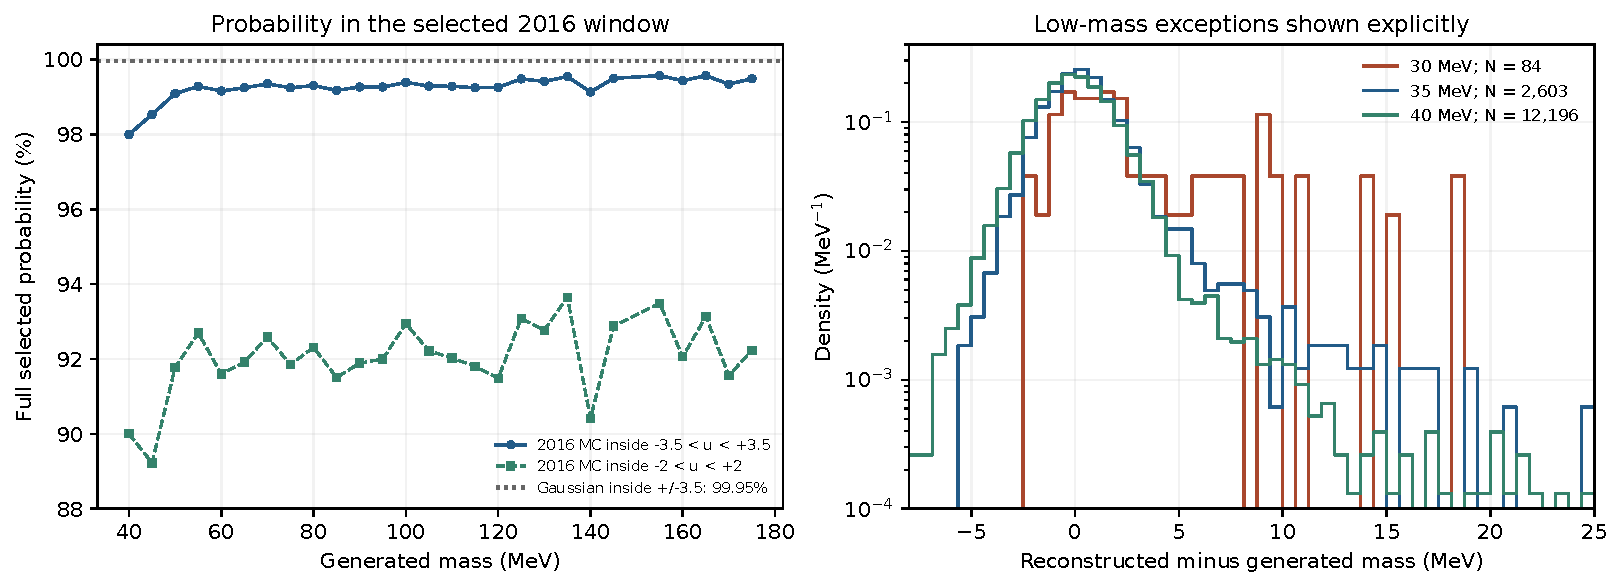
\includegraphics[width=\linewidth,height=3.3in,keepaspectratio]{../figures/shape_containment_and_low_mass.pdf}\end{center}
{\small\refstepcounter{figure}\textbf{Figure \thefigure. How to read the figure.} Left: the full selected probability inside $-3.5\le u\le+3.5$, the adopted 2016 fit and training-exclusion interval. The narrower $|u|<2$ fraction is a shape reference. A matched Gaussian has 99.95\% inside $|u|<3.5$. Right: the 30, 35 and 40 MeV histograms are shown without rescaling their displayed ranges. The two sparse low-mass samples are retained visibly rather than pooled into the primary shape comparison.}\par\medskip

The adopted window contains 98.00--99.57\% of the full selected MC probability across the primary 2016 samples. This is the geometric fraction of a signal template inside a specified interval. It is not a selection efficiency or a measured recovery fraction. Signal outside the excluded region can still enter the GP-training sidebands; a wider exclusion changes both the signal contamination and the available background information.

\textbf{30 MeV: no reliable fitted core.} Only 84 entries survive in the supplied histogram. The primary fit reaches its minimum-width bound, and only 34 of 64 resampling fits pass the locator checks. The binned mean is 34.10 MeV and the median is 31.81 MeV. Neither statistic makes the failed local Gaussian fit a reliable core measurement. Its attempted fit remains in the numerical ledger, but is not used for interpolation.

\textbf{35 MeV: a separate diagnostic.} This histogram has 2,603 entries. Its primary core center is 35.276 MeV and its mean is 35.695 MeV. Changing the pedestal-fit half-width from 1.5 to 2.0 reference widths changes the fitted core width from about 0.91 to 1.44 MeV. That sensitivity motivates keeping this sample outside the primary template prescription.

\textbf{40--175 MeV: the primary template domain.} All 27 available core fits and all their resampling fits pass. The 40 MeV sample remains in the comparison and has the largest common-shape discrepancy, so the low-mass qualification does not conceal the remaining shape change. No empirical template is extrapolated below 40 or above 175 MeV.

\textbf{Input checks.} Every analyzed histogram is a 400-bin TH1D on 0--0.25 GeV, converted once to 0--250 MeV. Its bins are 0.625 MeV wide; counts are nonnegative integers, variances equal counts, entries equal the bin sum, and underflow and overflow are zero. Generated masses come from the file names. The ROOT files have blank axis titles and no embedded fits; the supplied sample description provides the prompt/target-constrained and FEE provenance.

\clearpage\section*{Native central locations and widths}

All masses and widths are in MeV. Here $c$ is the fitted core center, SD is its conditional MC resampling error, $s$ is the fitted core width, and $F_2$ is the full selected fraction inside $c\pm2s$. ``Spread'' is the largest change in center across the four alternate local-fit definitions. The CSV retains more precision than this table.

\begin{center}\fontsize{8.5}{10.5}\selectfont\setlength{\tabcolsep}{3.1pt}
\begin{tabular}{rrrrrrrrrr}\toprule
$m$ & Entries & $c$ & $c-m$ & SD$(c)$ & $s$ & Median & Mean & $F_2$ [\%] & Spread\\\midrule
30 & 84 & -- & -- & -- & -- & 31.806 & 34.100 & -- & --\\
35 & 2,603 & 35.276 & $+0.276$ & 0.088 & 0.913 & 35.313 & 35.695 & 70.8 & 0.145\\
40 & 12,196 & 39.889 & $-0.111$ & 0.062 & 1.560 & 39.984 & 40.131 & 90.0 & 0.075\\
45 & 46,316 & 44.920 & $-0.080$ & 0.059 & 1.641 & 44.922 & 44.938 & 89.2 & 0.119\\
50 & 91,802 & 49.884 & $-0.116$ & 0.022 & 1.967 & 49.868 & 49.865 & 91.8 & 0.049\\
55 & 139,637 & 54.888 & $-0.112$ & 0.021 & 2.208 & 54.821 & 54.789 & 92.7 & 0.050\\
60 & 188,657 & 59.812 & $-0.188$ & 0.028 & 2.274 & 59.783 & 59.737 & 91.6 & 0.044\\
65 & 221,366 & 64.833 & $-0.167$ & 0.026 & 2.500 & 64.741 & 64.682 & 91.9 & 0.067\\
70 & 245,676 & 69.839 & $-0.161$ & 0.033 & 2.751 & 69.710 & 69.635 & 92.6 & 0.102\\
75 & 280,200 & 74.762 & $-0.238$ & 0.024 & 2.847 & 74.676 & 74.596 & 91.8 & 0.036\\
80 & 277,884 & 79.714 & $-0.286$ & 0.027 & 3.094 & 79.657 & 79.561 & 92.3 & 0.056\\
85 & 273,602 & 84.735 & $-0.265$ & 0.026 & 3.194 & 84.618 & 84.513 & 91.5 & 0.078\\
90 & 273,665 & 89.728 & $-0.272$ & 0.035 & 3.447 & 89.584 & 89.475 & 91.9 & 0.087\\
95 & 309,188 & 94.744 & $-0.256$ & 0.036 & 3.670 & 94.578 & 94.454 & 92.0 & 0.113\\
100 & 290,224 & 99.691 & $-0.309$ & 0.034 & 4.055 & 99.546 & 99.412 & 92.9 & 0.084\\
105 & 172,514 & 104.731 & $-0.269$ & 0.046 & 4.145 & 104.512 & 104.373 & 92.2 & 0.163\\
110 & 148,579 & 109.620 & $-0.380$ & 0.053 & 4.317 & 109.480 & 109.350 & 92.0 & 0.061\\
115 & 124,340 & 114.596 & $-0.404$ & 0.076 & 4.510 & 114.456 & 114.312 & 91.8 & 0.082\\
120 & 114,544 & 119.481 & $-0.519$ & 0.062 & 4.683 & 119.418 & 119.283 & 91.5 & 0.089\\
125 & 108,179 & 124.412 & $-0.588$ & 0.075 & 5.209 & 124.431 & 124.269 & 93.1 & 0.233\\
130 & 85,681 & 129.427 & $-0.573$ & 0.081 & 5.355 & 129.381 & 129.226 & 92.8 & 0.104\\
135 & 81,070 & 134.549 & $-0.451$ & 0.073 & 5.811 & 134.371 & 134.202 & 93.7 & 0.125\\
140 & 70,169 & 139.670 & $-0.330$ & 0.100 & 5.398 & 139.350 & 139.148 & 90.4 & 0.247\\
145 & 58,314 & 144.354 & $-0.646$ & 0.100 & 6.121 & 144.330 & 144.183 & 92.9 & 0.153\\
155 & 23,967 & 154.268 & $-0.732$ & 0.191 & 6.696 & 154.262 & 154.090 & 93.5 & 0.275\\
160 & 30,696 & 158.983 & $-1.017$ & 0.181 & 6.574 & 159.159 & 159.027 & 92.1 & 0.396\\
165 & 34,356 & 164.219 & $-0.781$ & 0.151 & 7.069 & 164.156 & 163.985 & 93.1 & 0.049\\
170 & 31,571 & 169.259 & $-0.741$ & 0.215 & 6.738 & 169.107 & 168.951 & 91.6 & 0.268\\
175 & 33,055 & 174.272 & $-0.728$ & 0.187 & 7.056 & 174.066 & 173.894 & 92.2 & 0.175\\
\bottomrule\end{tabular}\end{center}

The 30 MeV fit is invalid; the 35 MeV row is diagnostic and excluded from primary averages and interpolation. There is no 150 MeV input. The binned mean uses bin midpoints, and quantiles assume uniform probability within a bin. These histogram summaries cannot recover event-level locations.

The reference analysis-resolution curve used by the core locator is
\[
 \sigma_{\rm ref}=0.000380+0.0410m-0.270m^2+3.490m^3-11.11m^4,
 \qquad m,\sigma_{\rm ref}\ \hbox{in GeV}.
\]
It is retained as a documented comparison and locator convention. The MC fit window uses the empirical width $s(m)$, not this reference polynomial.


\clearpage\section*{From an MC shape to an observed-data fit}
\label{sec:method}

\textbf{One core-centered coordinate, two year-specific windows.} The local Gaussian fit supplies only the core center and width used to align the native histograms. It does not replace their tails. If $m$ lies between simulated masses $m_L$ and $m_R$, define $t=(m-m_L)/(m_R-m_L)$ and interpolate $c(m)$ and $s(m)$ linearly. For an analysis-bin edge $x$, evaluate
\[
 F_m(x)=(1-t)F_L\!\left(c_L+s_L\frac{x-c(m)}{s(m)}\right)
       +tF_R\!\left(c_R+s_R\frac{x-c(m)}{s(m)}\right).
\]
Each $F$ is the cumulative probability of a full selected native histogram, with piecewise-uniform probability within its bins. Analysis-bin probabilities are differences of $F_m$ at the edges. At an MC anchor the native histogram is recovered exactly. Its reconstructed displacement is already present; no second translation is added.

\begin{center}\begin{tabular}{lll}\toprule
Extraction & Signal-fit bins & GP-training bins\\\midrule
2016 MC & $|u|\le3.5$ & $|u|>3.5$\\
2021 MC & $-4\le u\le+3$ & $u<-4$ or $u>+3$\\
Gaussian reference & $|m_{\rm rec}-c_G|\le2.25\sigma_{\rm ref}$ & Exterior of the same interval\\\bottomrule
\end{tabular}\end{center}

Bin centers determine membership. The actual outer bin edges, selected bin counts and interpolation anchors are saved for every mass. The 2016 scan uses 1 MeV steps from 40 through 175 MeV; the combined scan uses 60 through 240 MeV. No 2016 template is extrapolated into the missing region above 175 MeV. In the 2016 MC scan, 97.93--99.58\% of the selected signal falls in the actual fitted bins. The remaining 0.42--2.07\% falls in training bins and is retained in injected samples. This small fraction can still affect background prediction.

\textbf{Two controls make the 2016 change interpretable.} The inherited Gaussian uses its original center, reference width and window. A second Gaussian control retains exactly that signal shape but adopts the new MC-centered fit/training window. The final method then replaces the Gaussian by the neighboring MC shape in that same window. The control separates the window change from the subsequent shape change; neither difference is solely a correction to the center.

For 2015 and 2016, the reference Gaussian center is the generated mass. For 2021 it retains the established shift,
\[
 c_G(m)=m-3.22433\,{\rm MeV}-2.21399\,{\rm MeV}\ln\!\left(\frac{m}{150\,{\rm MeV}}\right).
\]
Thus ``all Gaussian'' means the established v6.3.n reference, including its already shifted 2021 Gaussian. The Gaussian widths retain the archived resolution curves. The 2015/2016 reference Gaussians retain their historical normalization over the stored spectrum; MC probabilities always retain the full selected normalization, including any probability outside that spectrum.

The 2021 extraction uses the latest saved v16 target-constrained MC bank over 60--240 MeV and the same linear neighbor convention. The earlier 2021 samples used in the shape-comparison figures provide context for the displacement; their fitted parameters are not substituted for this production bank. Interpolation near the 2021 low-mass acceptance transition remains a model assumption.

\clearpage\section*{What do the fitted yield, upper limit and probability mean?}

The Gaussian process (GP) predicts the background in the excluded interval from the exterior bins. Its kernel amplitude and length scale are fixed to the archived mass-dependent values. Conditioning on the logarithms of positive bin counts, with variance $1/n$, gives a lognormal arithmetic mean $b$ and a correlated count-space covariance $V$. Empty training bins retain the archived log-target and variance conventions. The GP prediction is recomputed after each change of window and for every toy dataset; the kernel parameters are not reoptimized.

Write $V=LL^T$, including the inherited numerical regularization. In one campaign, the bin expectation is $\lambda_i=b_i+(L\theta)_i+A p_i$, where $p_i$ is the full selected signal probability in fit bin $i$. The constrained count likelihood is
\[
 -\ln\mathcal L(A,\theta)
 =\sum_{i\in{\rm fit}}\left[\lambda_i-n_i+n_i\ln\frac{n_i}{\lambda_i}\right]
  +\tfrac12\theta^T\theta .
\]
The $n_i=0$ logarithmic term is zero and every expected bin count must remain positive. The nuisance parameters allow correlated background changes penalized by the GP covariance. Their fitted background can differ from the initial GP mean. The likelihood uses the fit bins; exterior bins influence it through the GP constraint.

\textbf{The yield is signed for diagnosis.} The unconstrained estimate $\Ah$ can be negative. Its displayed error is the conditional curvature (Hessian) error after profiling the background. A positive MC-template yield refers to the full selected MC distribution, rather than only the probability inside the fitted interval. No fit-window renormalization is applied. A Gaussian yield describes that Gaussian model and need not measure an injected MC-shaped yield without calibration.

\textbf{The continuous curves are conditional profile limits.} For a tested nonnegative signal strength, the nuisance parameters are profiled again. The bounded likelihood-ratio denominator uses the free fit when its signal is positive and the background-only fit otherwise. The solver uses the inherited asymptotic sampling tails, with a background-mean Asimov profile, and solves $CL_s=0.10$. Thus the plotted curves are observed 90\% profile-$CL_s$ limits under the stated model and sampling approximation. They are not obtained by simply adding $1.64$ errors to $\Ah$.

\textbf{The displayed probability is local.} Define the signed likelihood root and its excess-only statistic by
\[
 r={\rm sign}(\Ah)\sqrt{2\,[\ln\mathcal L(\Ah,\widehat\theta)-\ln\mathcal L(0,\widehat\theta_0)]},
 \qquad q_0=\max(0,r)^2,\qquad p_0=\Phi[-\max(0,r)].
\]
Here $\Phi$ is the standard normal cumulative distribution. Deficits have displayed $p_0=0.5$. This asymptotic number refers to one mass and one fixed template. It does not include scanning masses, choosing two excess regions, or uncertainty in the estimated background source. The selected-point toy checks below test its behavior under a specified fixed background source.

The two 2016 examples are positive local maxima ranked by $q_0$, with the additional requirement that their fitted bins do not overlap. This selects 91 and 69 MeV. It is a way to show two distinct fitted regions, not an independence claim: their GP sidebands can still overlap. The same rule applied campaign by campaign selects 68 and 94 MeV in the combined scan.

\clearpage\section*{How are the years combined?}

\textbf{The combination shares a signal parameter and keeps separate backgrounds.} Let $\psi=\epsilon^2_{ee}/10^{-8}$ denote the inherited coupling-conversion coordinate. For campaign $y$, define $K_y(m)$ as the expected selected event yield per unit $\psi$. The combined likelihood uses
\[
 \lambda_{yi}=b_{yi}+(L_y\theta_y)_i+\psi K_y(m)p_{yi},
 \qquad -\ln\mathcal L_{\rm joint}=\sum_y[-\ln\mathcal L_y].
\]
The background constraints are independent between campaigns, while $\psi$ is common. Local probabilities follow from this joint likelihood; they are not multiplied between years. The signal MC defines $p_{yi}$, and the inherited conversion defines $K_y$. A common signal fit can move individual campaign backgrounds differently.

\begin{center}\begin{tabular}{ll}\toprule
Generated-mass range & Campaigns in every compared policy\\\midrule
60--100 MeV & Full 2015, full 2016, 2021 10\%\\
101--175 MeV & Full 2016, 2021 10\%\\
176--240 MeV & 2021 10\% only\\\bottomrule
\end{tabular}\end{center}

Keeping the same campaign support is essential for the shape comparison. In particular, the old 2016 Gaussian availability through 180 MeV is truncated to 175 MeV here for all policies, because the new MC bank stops there. Above 175 MeV the two MC-based combinations must coincide exactly. Boundaries can produce visible changes because a dataset ceases to contribute.

\textbf{The conversion is inherited, rather than remeasured.} At generated mass $m$, the archived native spectrum provides a local event density $\rho_y(m)$ averaged across $m\pm1.64\sigma_{{\rm ref},y}(m)$, using fractional overlap with the native bins. With the archived effective radiative fraction $f_{{\rm rad},y}$,
\[
 K_y(m)=10^{-8}\frac{3\pi}{2\alpha}\,m\,f_{{\rm rad},y}\,\rho_y(m),\qquad \alpha=1/137,
\]
where mass and density use reciprocal units. This calculation stays centered at the generated mass for every template policy. Moving the reconstructed signal core therefore does not silently move the conversion window. The per-mass values are supplied in \texttt{results/normalization.csv}.

Above $2m_\mu=211.316749$ MeV, the displayed coupling limit retains the earlier visible-decay multiplier
\[
 \epsilon^2_{\rm displayed}=10^{-8}\psi\left[1+\sqrt{1-4r_\mu}\,(1+2r_\mu)\right],
 \qquad r_\mu=(m_\mu/m)^2.
\]
Below this threshold the multiplier is one. Both the unmultiplied $ee$ coordinate and the historical displayed value are saved. This inherited convention, including its selected-spectrum density and radiative fraction, supports an internally consistent comparison. A new efficiency, acceptance, detector calibration or branching-model validation has not been derived from the supplied histograms.

The plotted curves keep MC shape, core location, width, GP kernel settings and the conversion inputs fixed. Their statistical comparison does not include uncertainties in those ingredients. A joint observed upper limit need not be smaller than each individual observed limit, because the datasets fluctuate and share a constrained signal strength.
% Observed results only. The root report supplies inference definitions,
% fixed-source null checks, the preamble, and the running figure counter.
\clearpage\section*{2016 extraction: separate the window and template changes}

The 2016 scan compares three choices on the same spectrum: the inherited Gaussian in its original window; that same Gaussian in the MC-centered $[-3.5,+3.5]u$ fit and training-exclusion interval; and the neighboring MC template in that interval. The intermediate choice isolates the window change before changing the signal shape.

\begin{center}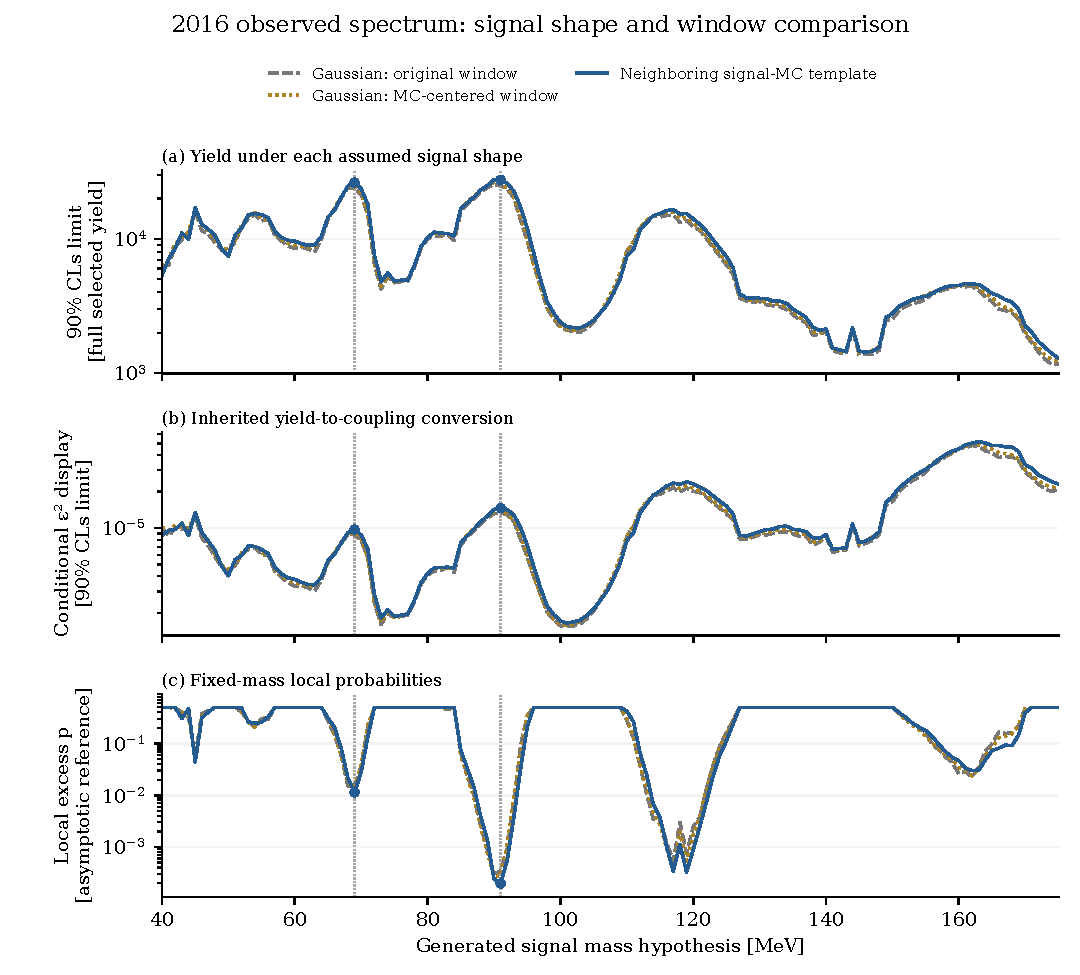
\includegraphics[width=\linewidth,height=4.8in,keepaspectratio]{../figures/extraction_2016_scan.pdf}\end{center}
{\small\refstepcounter{figure}\textbf{Figure \thefigure. How to read the figure.} Gray: the inherited Gaussian centered at the generated mass, with the original $\pm2.25\sigma_{\rm ref}$ interval. Gold: the same Gaussian with the MC-centered fit and exclusion interval. Blue: the neighboring MC template in that interval. Top: observed 90\% profile-CLs limits on each assumed shape's full selected yield. Middle: the inherited conditional conversion to the $\epsilon^2$ display. Bottom: fixed-mass asymptotic excess probabilities. Blue points identify the two regions shown next. The Gaussian and MC curves describe different signal-shape assumptions; their limits are not interchangeable calibrations of an MC-shaped signal.}\par\medskip

Across the 136 tested masses from 40 to 175 MeV, changing only the window changes the upper limit by a median $+3.6\%$, with a range of $-1.3\%$ to $+10.4\%$. Replacing the Gaussian with MC at that fixed window adds a median $+3.2\%$, with a range of $-14.8\%$ to $+20.6\%$. These summarize the observed scan, not an uncertainty distribution.

The smallest local asymptotic probability moves from $3.08\times10^{-4}$ at 90 MeV for the original Gaussian to $2.75\times10^{-4}$ at 91 MeV for the window control, then $1.96\times10^{-4}$ at 91 MeV for MC. These are local references selected from a mass scan. The fixed-source null checks are discussed separately; none of these minima is a global discovery probability.

\clearpage\section*{2016: the strongest selected region, at 91 MeV}

The MC fit returns a signed full selected yield of $20{,}201\pm5{,}699$ events. Its core is at 90.731 MeV with width 3.492 MeV. The actual fitted bins cover 78.50--103.00 MeV and contain 99.27\% of the selected template probability. The signal yield still refers to the complete template.

\begin{center}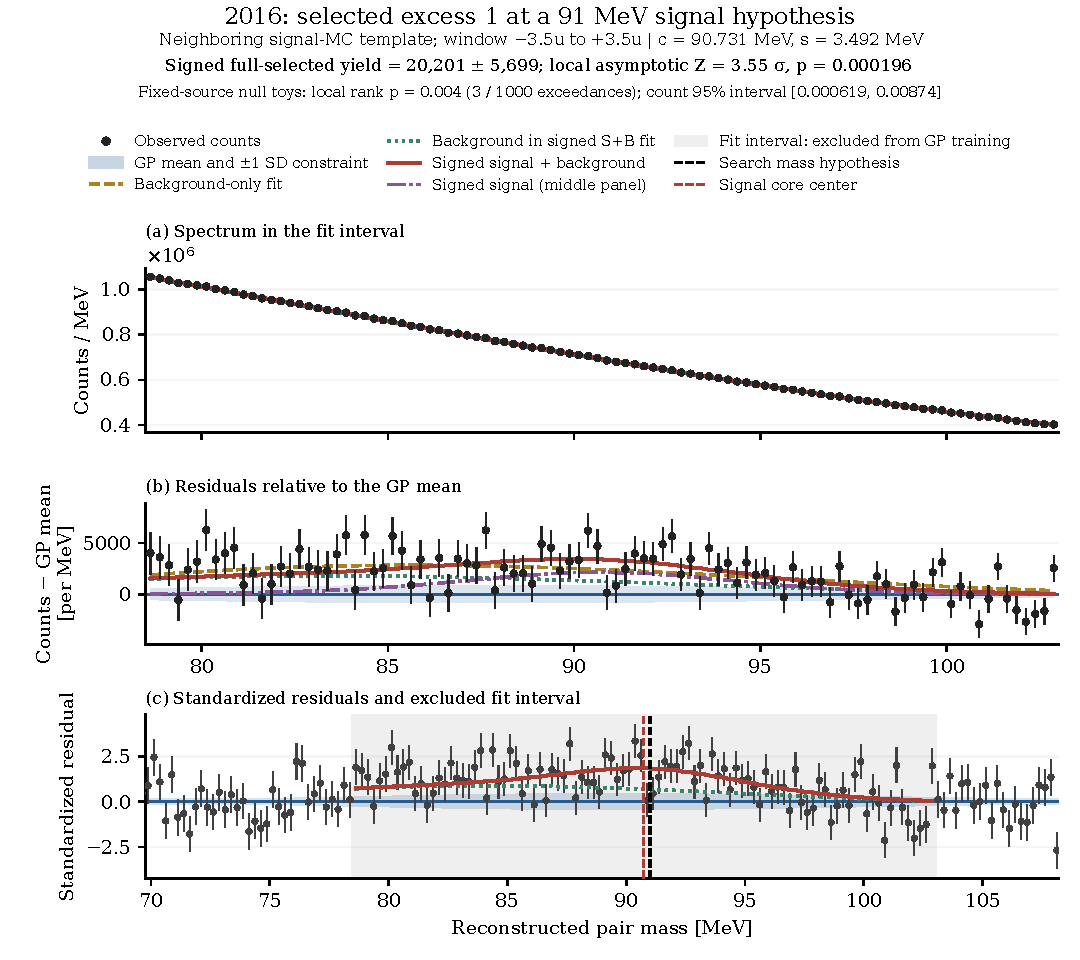
\includegraphics[width=\linewidth,height=5.7in,keepaspectratio]{../figures/extraction_2016_excess_1.pdf}\end{center}
{\small\refstepcounter{figure}\textbf{Figure \thefigure. How to read the figure.} Black points are observed counts with square-root-count errors. Blue is the GP sideband prediction with its marginal one-standard-deviation constraint band. Gold is the profiled background-only fit; green is the background component of the signed signal-plus-background fit; red is its total. The middle panel subtracts the GP mean and shows the signed signal in purple. The bottom panel standardizes residuals by $\sqrt{b_{\rm GP}+V_{{\rm GP},ii}}$ and shades the excluded fit interval. The black and red vertical lines mark the generated hypothesis and MC core. Profiled curves appear only in the fitted bins. The blue band is a background constraint, and the correlated residuals are not independent significance measurements.}\par\medskip

At this same 91 MeV hypothesis, the upper yield limit is 25,048 events for the original Gaussian, 26,031 for the Gaussian window control, and 27,505 for MC. The corresponding local asymptotic significances are 3.40, 3.46 and 3.55. The null-toy annotation provides a separate conditional reference: three of 1,000 toys exceed the observed MC statistic, giving the add-one rank $4/1001$. Its interpretation and finite-sample interval are treated in the null-check discussion.

\clearpage\section*{2016: the second distinct region, at 69 MeV}

The second displayed region, at 69 MeV, is the strongest remaining local maximum with fitted bins disjoint from the 91 MeV region. The 117 and 119 MeV maxima have smaller local probabilities but overlap that fitted interval; they remain visible in the full scan.

\begin{center}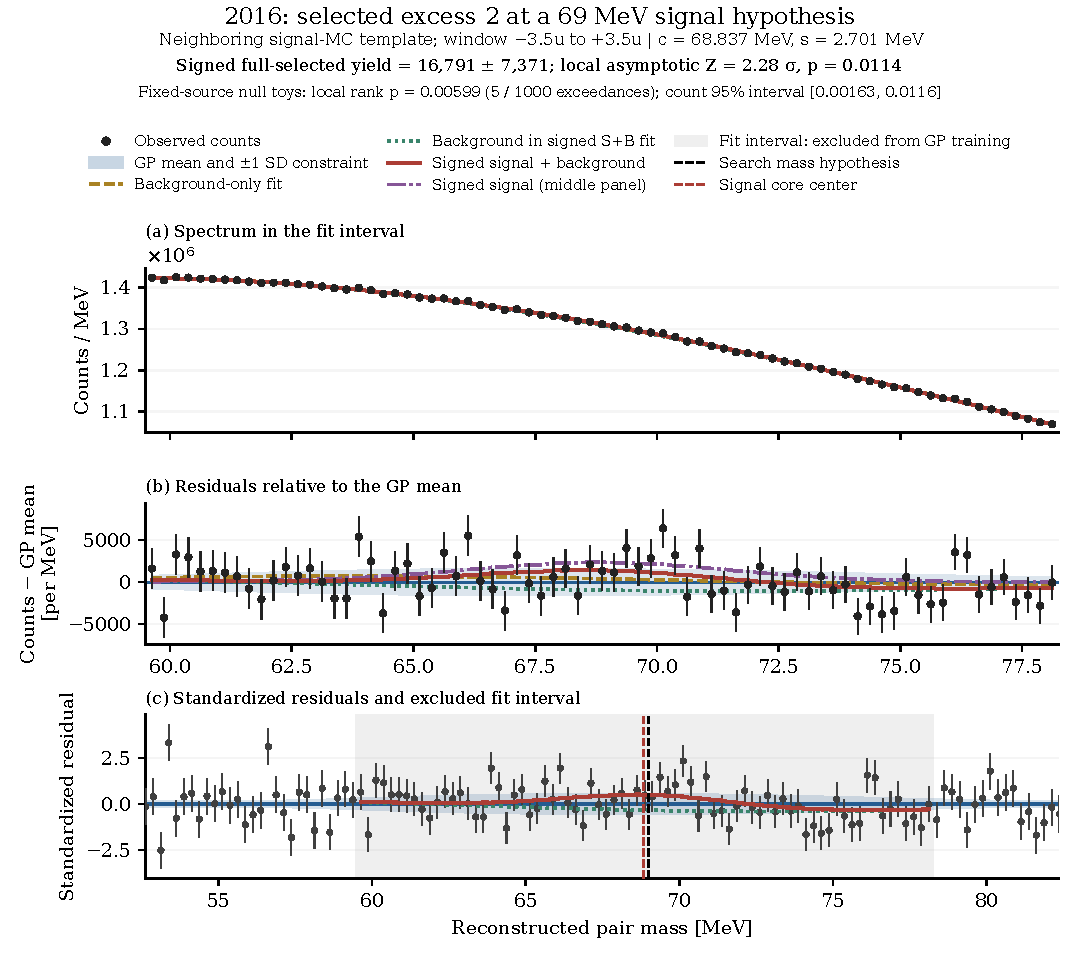
\includegraphics[width=\linewidth,height=5.05in,keepaspectratio]{../figures/extraction_2016_excess_2.pdf}\end{center}
{\small\refstepcounter{figure}\textbf{Figure \thefigure. How to read the figure.} The three panels and curves use the same definitions as the preceding fit: observed spectrum, residuals relative to the GP prediction, and standardized residuals including neighboring sidebands. The actual fit and training-exclusion interval is 59.50--78.25 MeV. The template core is at 68.837 MeV with width 2.701 MeV; 99.29\% of its selected probability lies in the fitted bins. Its quoted yield retains full selected normalization. The two displayed fit intervals are disjoint, but their GP sidebands overlap, so they are not independent tests.}\par\medskip

The fitted MC yield is $16{,}791\pm7{,}371$ events, with a local asymptotic probability of 0.0114. At 69 MeV, the upper yield limit changes from 23,750 events for the original Gaussian to 24,800 for the Gaussian window control and 26,285 for MC. The MC conditional coupling display is $\epsilon^2_{90}=9.74\times10^{-6}$.

Five of the 1,000 fixed-source null toys exceed the observed statistic, giving the add-one rank $6/1001$. This rank and its interval describe the specified null source at this mass. Choosing the region using the observed scan is not included in that probability. The report's null-check discussion explains the distinction between these ranks and the dense asymptotic curves.

\clearpage\section*{Combine the campaigns with three signal prescriptions}

The combined comparison starts from the established Gaussian analysis, replaces 2021 with neighboring MC, then also replaces 2016 with neighboring MC. The 2015 Gaussian is retained throughout. The all-Gaussian reference \emph{already uses the established logarithmic core shift for 2021}.

\begin{center}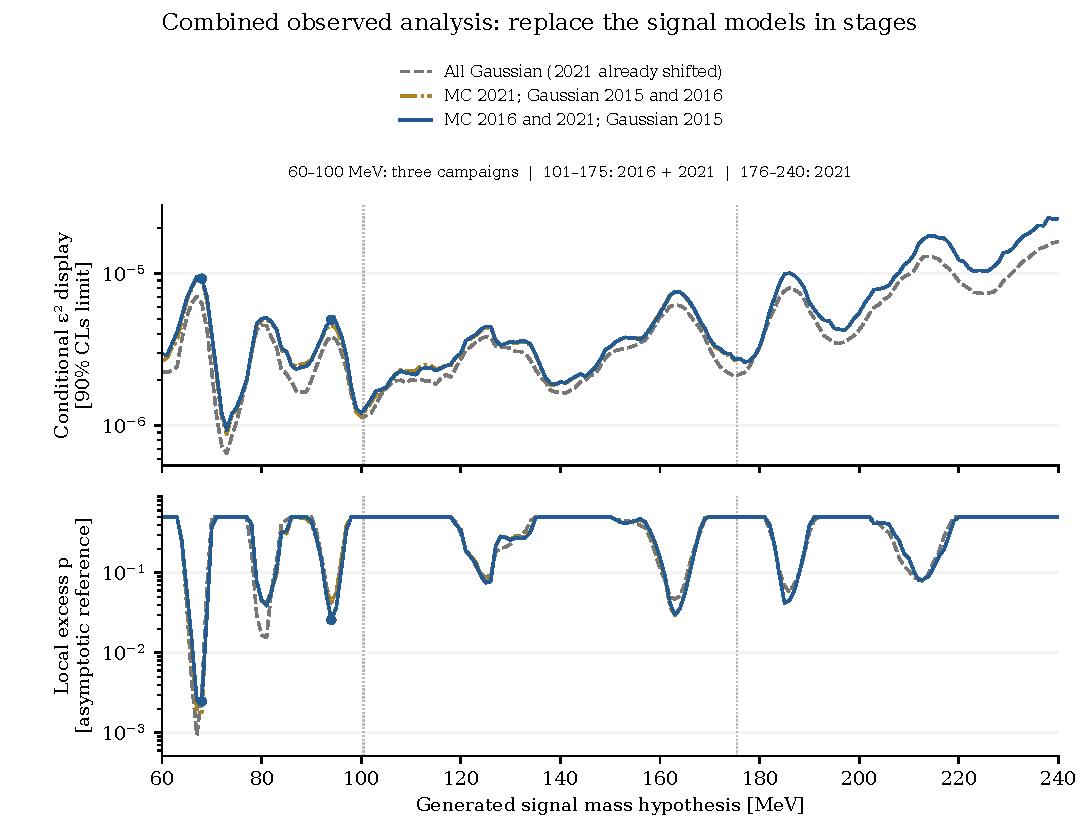
\includegraphics[width=\linewidth,height=4.2in,keepaspectratio]{../figures/extraction_combined_comparison.pdf}\end{center}
{\small\refstepcounter{figure}\textbf{Figure \thefigure. How to read the figure.} Top: conditional observed 90\% profile-CLs limits in the inherited $\epsilon^2$ display. Bottom: local asymptotic excess probabilities. The two MC choices use $[-4,+3]u$ for 2021, and the final choice also uses $[-3.5,+3.5]u$ for 2016. Fit and GP-exclusion intervals change together. All curves use the same campaign support: 2015, 2016 and 2021 at 60--100 MeV; 2016 and 2021 at 101--175 MeV; and 2021 alone at 176--240 MeV. Vertical dotted lines mark these transitions. The two MC curves coincide above 175 MeV. Blue points mark the selected combined regions.}\par\medskip

\begin{center}\small\begin{tabular}{lrrr}\toprule
Combined signal prescription & Minimum at [MeV] & Local $p_0$ & Local $Z$\\\midrule
All Gaussian; 2021 shifted & 67 & $9.33\times10^{-4}$ & 3.11\\
2021 MC; 2015/2016 Gaussian & 68 & $1.81\times10^{-3}$ & 2.91\\
2016/2021 MC; 2015 Gaussian & 68 & $2.48\times10^{-3}$ & 2.81\\
\bottomrule\end{tabular}\end{center}

Thus the strongest combined local feature moves by 1 MeV and becomes less significant under the MC prescriptions. At the common 68 MeV hypothesis, the three upper-limit displays are $(6.35,\,9.05,\,9.26)\times10^{-6}$, respectively. The second selected combined region is at 94 MeV, with final-model $p_0=0.0257$ and $\epsilon^2_{90}=4.97\times10^{-6}$. These observed-selected local results retain the inference qualifications given in the method and null-check sections.

\clearpage\section*{Which campaign shapes the combined result?}

The common-coupling fit uses each campaign's own observations, background constraint and signal template. Individual excesses therefore need not reinforce one another at the same generated mass. The individual curves below help explain the combined result without treating their probabilities as quantities to multiply.

\begin{center}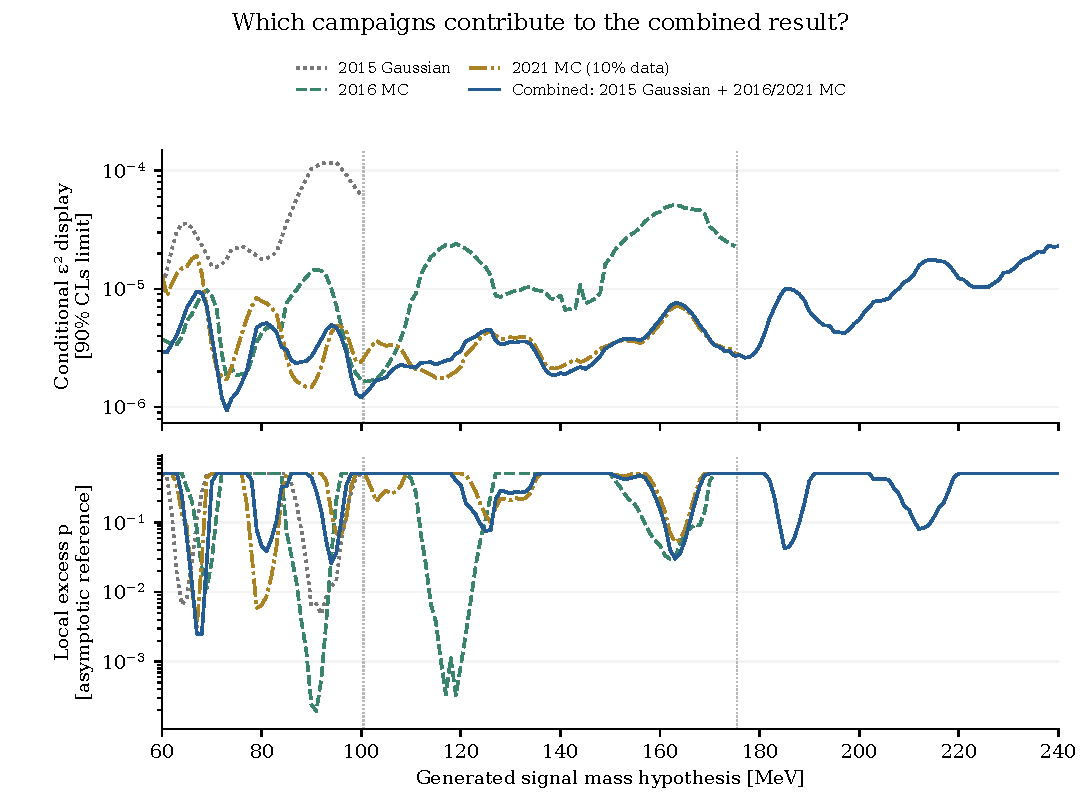
\includegraphics[width=\linewidth,height=5.15in,keepaspectratio]{../figures/extraction_campaign_contributions.pdf}\end{center}
{\small\refstepcounter{figure}\textbf{Figure \thefigure. How to read the figure.} Gray: the retained 2015 Gaussian. Green: the shifted 2016 MC template. Gold: the shifted 2021 MC template using the 10\% observed spectrum. Blue: their common-coupling profile combination, with separate GP constraints. Top: each conditional upper-limit display; bottom: each local asymptotic excess probability. The individual curves stop at their prescribed domain boundaries. Above 175 MeV, the combined curve is the 2021 curve. An observed combined upper limit need not be below every individual observed limit because the common signal parameter must describe all included datasets.}\par\medskip

At 91 MeV, the signed likelihood roots are $+2.47$ for the 2015 Gaussian, $+3.55$ for 2016 MC, and $-1.58$ for 2021 MC. The combined root is only $+0.59$, corresponding to local $p_0=0.277$. The strongest 2016 feature consequently does not become the strongest combined feature. A deficit in one campaign is relevant to the joint likelihood even though its one-sided excess probability is displayed as 0.5.

At 68 MeV, all three signed roots are positive: $+0.64$, $+2.03$ and $+1.90$, respectively. Their common-coupling fit gives the final model's largest combined excess statistic, with local $Z=2.81$. These comparisons describe compatibility with one common signal strength; they do not independently qualify the inherited conversion or supply a global mass-search calibration.

\clearpage\section*{How much do the combined upper limits change?}

The ratio view separates the large effect of replacing the 2021 Gaussian from the additional effect of updating 2016. Every ratio compares limits at the same generated mass, with the same included campaigns and coupling conversion.

\begin{center}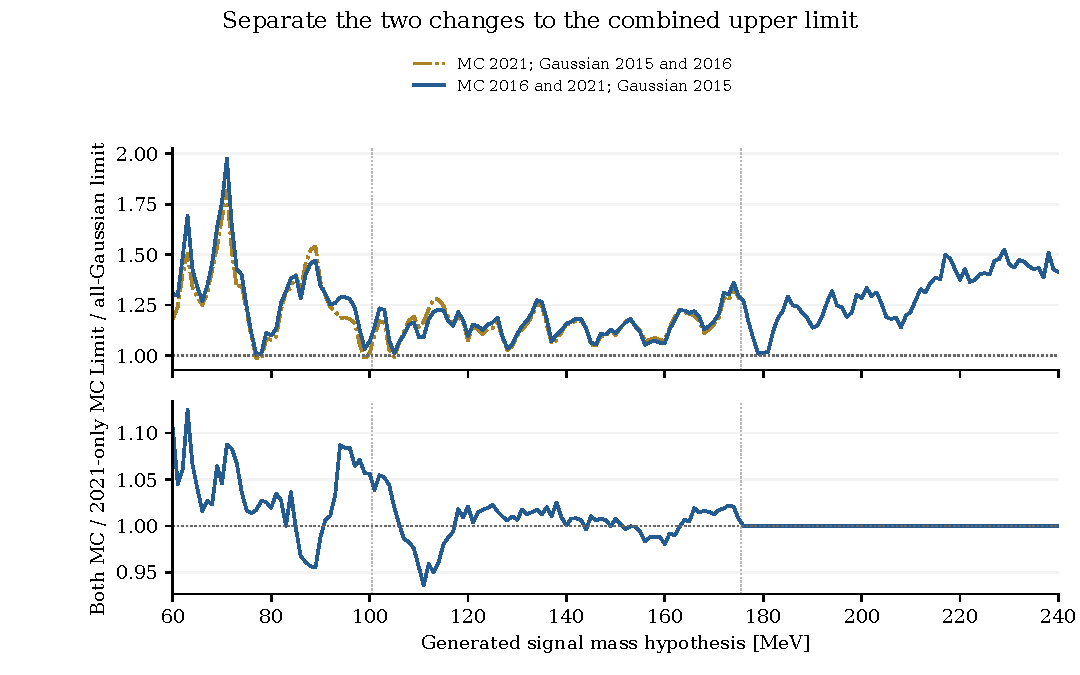
\includegraphics[width=\linewidth,height=4.25in,keepaspectratio]{../figures/extraction_combined_ratios.pdf}\end{center}
{\small\refstepcounter{figure}\textbf{Figure \thefigure. How to read the figure.} Top: each MC-based combined upper limit divided by the all-Gaussian combined limit. Bottom: the final model divided by the model that changes only 2021. One means no change; a value below one is a smaller conditional upper limit. The lower ratio is exactly one above 175 MeV because 2016 no longer contributes. These changes include both the assumed signal shape and its fit/training interval. They are not efficiency estimates or uncertainty bands.}\par\medskip

Across all 181 combined hypotheses from 60 to 240 MeV, replacing only 2021 changes the upper limit by a median $+19.5\%$, with a range from $-2.3\%$ to $+81.7\%$. Replacing both 2016 and 2021 changes it by a median $+21.8\%$ relative to the all-Gaussian reference, with a range from $+0.3\%$ to $+97.6\%$. The largest ratios occur at 71 MeV. These are descriptive summaries of the scanned observed limits; they are not repeated-experiment averages.

To isolate the added 2016 change, restrict attention to 60--175 MeV, where 2016 participates. Relative to the 2021-only MC result, adding 2016 MC changes the limit by a median $+1.3\%$, with a range from $-6.4\%$ at 111 MeV to $+12.5\%$ at 63 MeV. The change can have either sign because the signal shape and GP sidebands interact with the observed fluctuations.

\textbf{What the comparison establishes.} The final prescription has a defined shifted MC shape and exclusion interval for each of 2016 and 2021, while preserving the 2015 Gaussian. Its observed upper limits are generally higher than those from the inherited Gaussian comparison. A smaller local probability or a smaller limit would not, by itself, establish a better-calibrated procedure. The conditional conversion, the asymptotic limit construction and the finite null checks remain separate qualifications of the inference.

\clearpage\section*{Check the local probabilities with fixed-source backgrounds}

For each campaign, the archived GP arithmetic-mean spectrum is held fixed as the Poisson background source. Each toy fluctuates every stored analysis bin independently. The extraction then rebuilds its GP constraint from the toy's sidebands and profiles the same likelihood as for the observations. These toys do not draw new GP functions or retune the kernel. They test a conditional procedure for this source.

There are 1,000 background toys at each selected 2016 mass and at the combined 68 MeV mass. At 68 MeV the three methods receive the same toy counts; campaign draws are independent. At the two 2016 masses the same background draws are reused. For $k$ toys with $q_0$ at least as large as observed, the displayed rank is $(k+1)/1001$. The interval below is the exact two-sided 95\% Clopper--Pearson interval for the underlying exceedance probability.

\begin{center}\small\begin{tabular}{llrrrr}\toprule
Scope & Method/mass & Asymptotic $p_0$ & $k/1000$ & Add-one rank & 95\% interval\\\midrule
2016 & MC, 91 MeV & 0.000196 & 3 & 0.00400 & [0.00062, 0.00874]\\
2016 & MC, 69 MeV & 0.01136 & 5 & 0.00599 & [0.00163, 0.01163]\\
Combined & Gaussian, 68 MeV & 0.00317 & 0 & 0.00100 & [0, 0.00368]\\
Combined & 2021 MC, 68 MeV & 0.00181 & 0 & 0.00100 & [0, 0.00368]\\
Combined & Both MC, 68 MeV & 0.00248 & 0 & 0.00100 & [0, 0.00368]\\\bottomrule
\end{tabular}\end{center}

\textbf{The 91 MeV discrepancy is visible in the null mean.} At 91 MeV, the mean signed likelihood root is $+0.656$, with standard deviation 0.969. A background-only source therefore produces a positive fitted signal on average at this location. This explains why a standard-normal asymptotic reference can make the observed fit look more unusual than it does under this fixed source. The mean is a property of the specified background source and extraction; it is not subtracted from the observed result.

At 69 MeV the mean root is $-0.188$ with standard deviation 0.981. At combined 68 MeV the means are $-0.252$, $-0.225$ and $-0.211$ for all Gaussian, 2021 MC only and both MC, with standard deviations 0.967, 0.985 and 0.985. These means and spreads answer a different question from the signal response when MC events are added.

\textbf{Zero exceedances do not mean zero probability.} The 1,000 combined toys cannot distinguish the three tail probabilities at this precision. Their common upper interval endpoint is 0.00368. No numerical ordering of the three methods is inferred from the zero counts.

All these masses were chosen after examining the observed scans. Neither the asymptotic column nor the fixed-mass toy rank accounts for that search. A global probability would require repeating the full mass search and the same selection rule in each background toy, which was not done. The toy intervals quantify finite-ensemble uncertainty at the displayed mass, conditional on the fixed source; they do not cover uncertainty in the true background shape.

\clearpage\section*{Compare upper endpoints for the same injected signal}

The continuous Gaussian and MC profile curves fit different signal distributions. To compare their response to one specified signal, this additional selected-point study injects the full neighboring MC distribution for 2016 and 2021, with the retained Gaussian for 2015, into every method's background toys. The common expected strength is $\psi$; each campaign receives mean signal $\psi K_y$. All stored-bin and below/above-support categories are drawn, without renormalizing into the fitted interval. Realized counts fluctuate around these expected yields.

For each mass and trial strength, 200 calibration toys are fit by all three methods. The backgrounds are independent of the 1,000-toy null check. Within this calibration, methods share exactly the same background and signal draws, and increasing strengths add independent Poisson increments to the preceding signal draw. The scale $s_0$ is the Gaussian-reference error on the fixed background mean, independent of the observed fitted yield. The tested strengths are
\[
 \psi/s_0\in\{0,0.5,1,2,3,4,5,6,8,10,12,16\}.
\]
For each method, compare its signed observed fitted strength to the signed fitted strengths of the injected toys:
\[
 p_\psi=\frac{1+\#\{\widehat\psi_{\rm toy}\le\widehat\psi_{\rm obs}\}}{201}.
\]
Retain a trial strength if $p_\psi>0.10$. The table gives the largest accepted point and the next tested point, which is rejected. No interpolation between them is claimed. This is a one-sided finite-grid rank inversion, a different construction from the profile-$CL_s$ curves.

\begin{center}\small\begin{tabular}{llrr}\toprule
Scope, mass [MeV] & Extraction & Largest accepted & Next rejected\\
& & \multicolumn{2}{c}{$\epsilon^2$ in units of $10^{-6}$}\\\midrule
2016, 69 & Gaussian & 7.638 & 10.184\\
2016, 69 & Gaussian, new window & 7.638 & 10.184\\
2016, 69 & MC & 7.638 & 10.184\\
2016, 91 & Gaussian & 11.385 & 14.231\\
2016, 91 & Gaussian, new window & 11.385 & 14.231\\
2016, 91 & MC & 11.385 & 14.231\\
Combined, 68 & All Gaussian & 9.501 & 12.668\\
Combined, 68 & 2021 MC only & 9.501 & 12.668\\
Combined, 68 & 2016 + 2021 MC & 7.917 & 9.501\\\bottomrule\end{tabular}\end{center}

All nine accepted sets are nonempty, contain no holes on the tested grid and end below its largest strength. At 69 MeV the three methods share the largest accepted full 2016 yield of 20,617 events, with 27,489 events rejected at the next grid point. At 91 MeV the corresponding values are 21,405 and 26,756 events. Equality on this grid does not establish equality of continuous endpoints.

At combined 68 MeV the both-MC method rejects $6s_0$ with $p_\psi=18/201=0.0896$, while the other methods still accept that point. With only 200 calibration toys, this crossing is close to the 0.10 decision threshold. The apparent improvement in the discrete MC endpoint is therefore a conditional, finite-grid observation, not a precise sensitivity gain. It can coexist with a larger profile limit because the latter treats each extraction model's own signal as the hypothesis.

The 21,600 calibration fits preserve their complete signed-yield rows, rank counts, accepted sets, input-draw hashes and full-signal partitions. This targeted study does not establish 90\% coverage across the mass scan: it has no independent injected-signal evaluation ensemble and explores one estimated background source. The full continuous scans remain clearly labeled conditional profile diagnostics.

\clearpage\section*{What is established, and how can it be reproduced?}

The smeared 2016 samples support a small downward core displacement and a signal shape with tails that a Gaussian does not reproduce. A neighboring-MC template retains those features and gives a defined interpolation over 40--175 MeV. Using the specified core-centered windows produces the observed scans and the combined comparisons in this note. The fixed-source check also identifies a positive background-only fit bias at 91 MeV, so its asymptotic probability should not be read as an empirically calibrated significance.

The selected-point common-signal inversion provides a direct comparison of methods under one injected MC hypothesis. It includes signal in the training bins and outside the stored spectrum, and distinguishes expected yield from the realized Poisson signal. Its coarse grid and finite calibration sample are shown explicitly. Extending that calibration across masses and evaluating it on independent signal-injected samples would be required before treating it as a validated full-scan limit procedure.

\textbf{Frozen sources.} The package contains the 29 supplied 2016 ROOT histograms, extracted arrays and original shape-fit ledgers; the latest archived v16 target-constrained 2021 MC bank; archived observed spectra, resolution curves, kernel settings and conversion inputs; and the fixed GP-mean toy sources. There are 168 frozen input files in \texttt{provenance/input\_manifest.sha256}. The unsmeared 2016 histograms are not used in the extraction. Source comparisons to earlier versions are preserved as numerical inputs rather than dependencies on another working directory.

\textbf{Numerical checks.} The observed ledger has 1,354 rows: 992 fresh fits and 362 unchanged 2021 individual rows reused from v6.3.8. Independent checks verify input hashes, template normalization and anchor closure, fit/training geometry, selected regions, joint likelihood factorization, and targeted likelihood/Hessian replays. The inherited comparisons agree to numerical precision on the common campaign domain; 176--180 MeV is deliberately outside the old joint comparison because the campaign content has changed. All 5,000 null-toy fits and 21,600 injected calibration fits pass the saved numerical criteria.

\textbf{Portable rebuild.} From the package root, run \texttt{bash rebuild.sh}. The default reuses signature-checked numerical checkpoints; \texttt{bash rebuild.sh --fresh} regenerates the new observed fits and both toy studies. The 2021 individual rows are deliberately reused in either mode, with independent direct checks. Two local processes and one numerical thread per process are used. Python package versions and the LaTeX compiler are recorded in \texttt{provenance/runtime.json}. All figures are vector PDFs with PNG companions, and the LaTeX source uses the same article layout, typography, running header and explanatory captions as the v6.3.n notes.

The main numerical entry points are \path{scripts/run_scan.py}, \path{scripts/run_local_checks.py} and \path{scripts/run_rank_limits.py}. Tables and selected-fit arrays are under \texttt{results}; independent checks and PDF review records are under \texttt{qa}. The package manifest identifies the delivered files. Previous reports are preserved separately.

\textbf{Scope.} MC resampling errors describe finite simulation statistics. Core-definition changes describe sensitivity to the locator. Window containment describes geometry. Fitted response describes how the extraction reacts to injected signal. Local ranks describe one fixed source and mass. None of these quantities alone is a detector efficiency, a scan-wide probability or a complete uncertainty on a physical exclusion.
\clearpage\section*{Native signal-MC catalogue: 30--75 MeV}
\begin{center}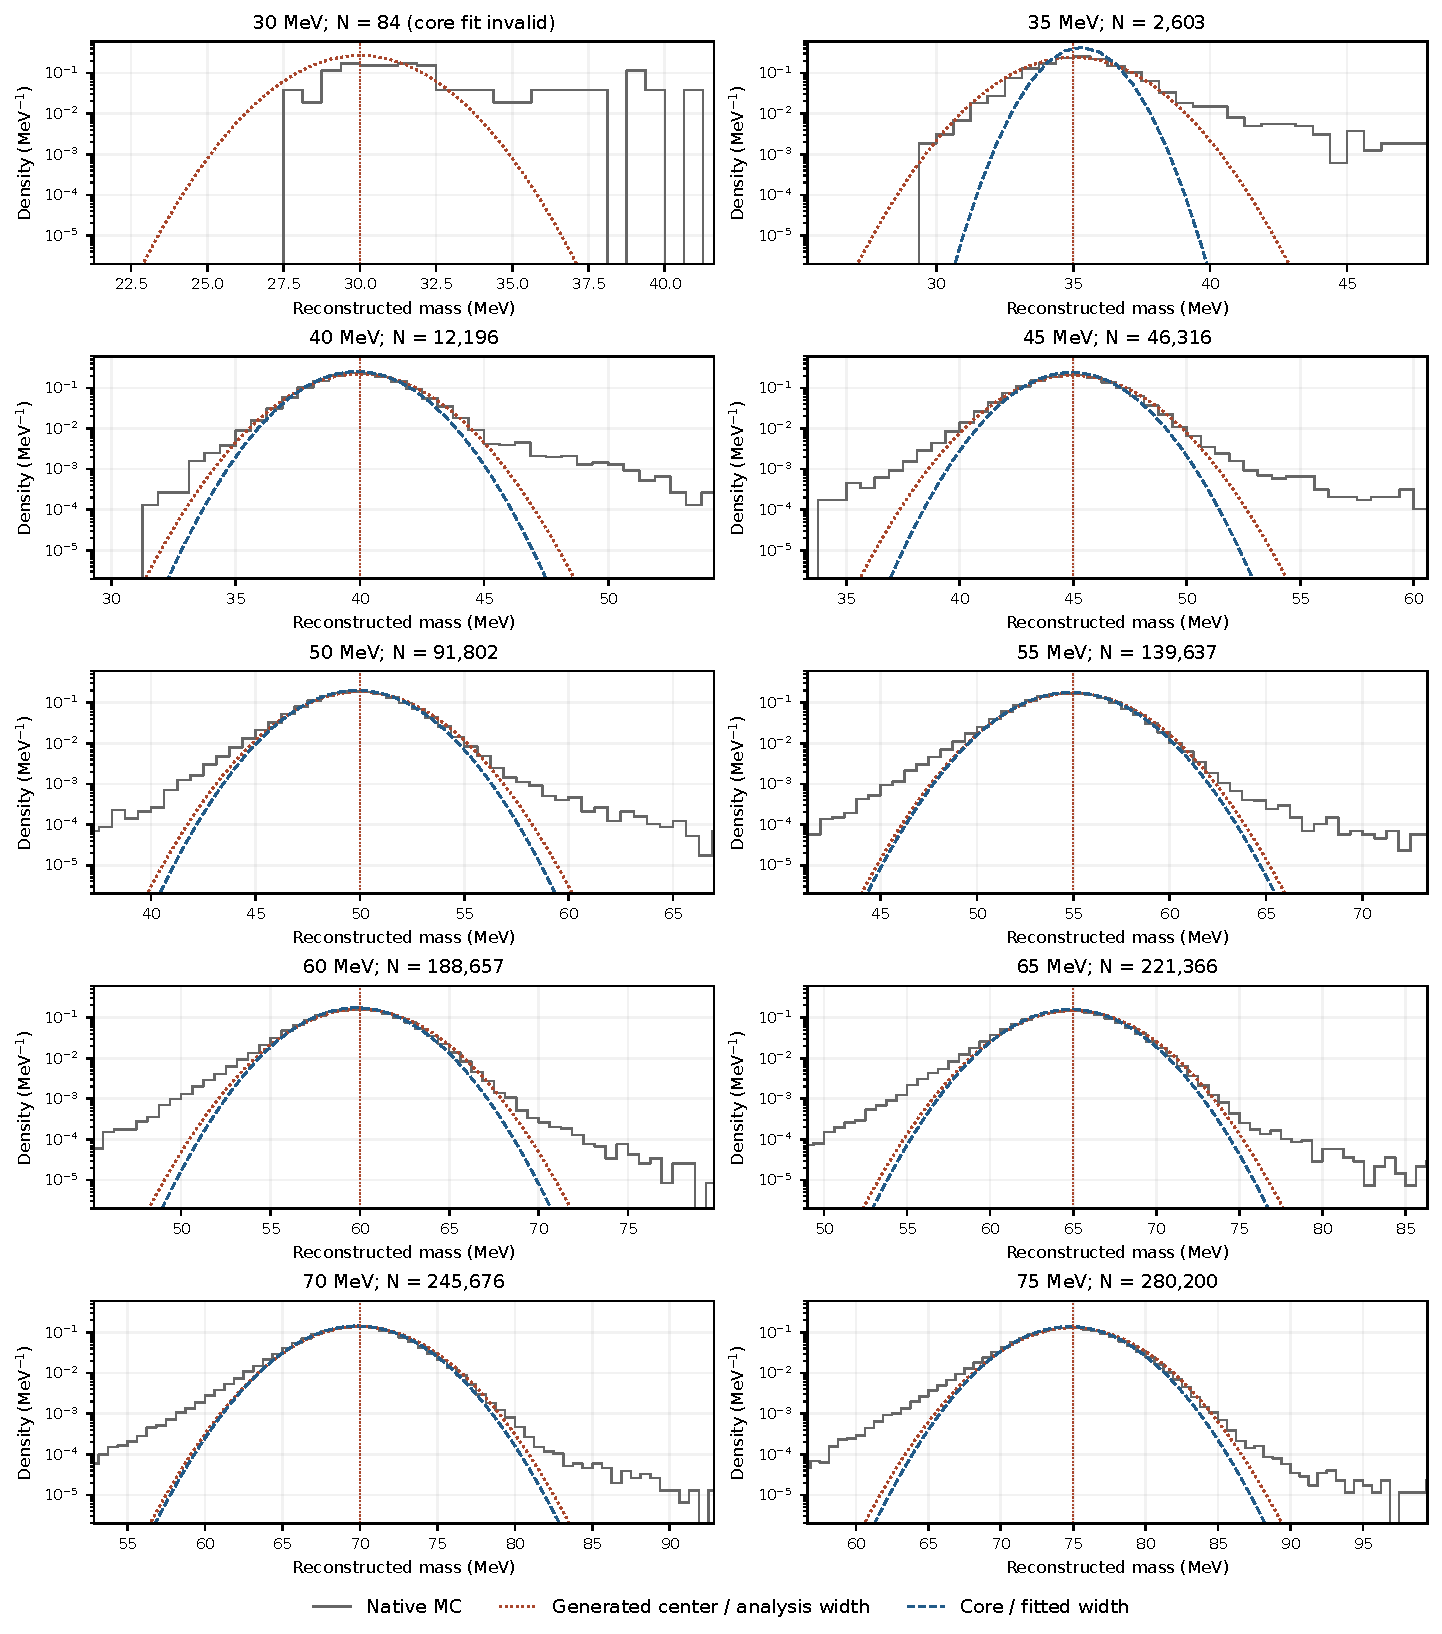
\includegraphics[width=\linewidth,height=6.65in,keepaspectratio]{../figures/shape_catalogue_1.pdf}\end{center}
{\small\refstepcounter{figure}\textbf{Figure \thefigure. How to read the figure.} Each panel shows the native MC with full selected normalization. Red dotted: a unit-area Gaussian at the generated mass with the reference analysis width. Blue dashed: a unit-area Gaussian at the fitted core with its fitted width. They are comparison shapes, rather than the local Gaussian component plus pedestal shown earlier. No blue curve is shown for the invalid 30 MeV core. The logarithmic axis exposes tails, and the displayed range does not change the normalization.}\par\medskip

\clearpage\section*{Native signal-MC catalogue: 80--125 MeV}
\begin{center}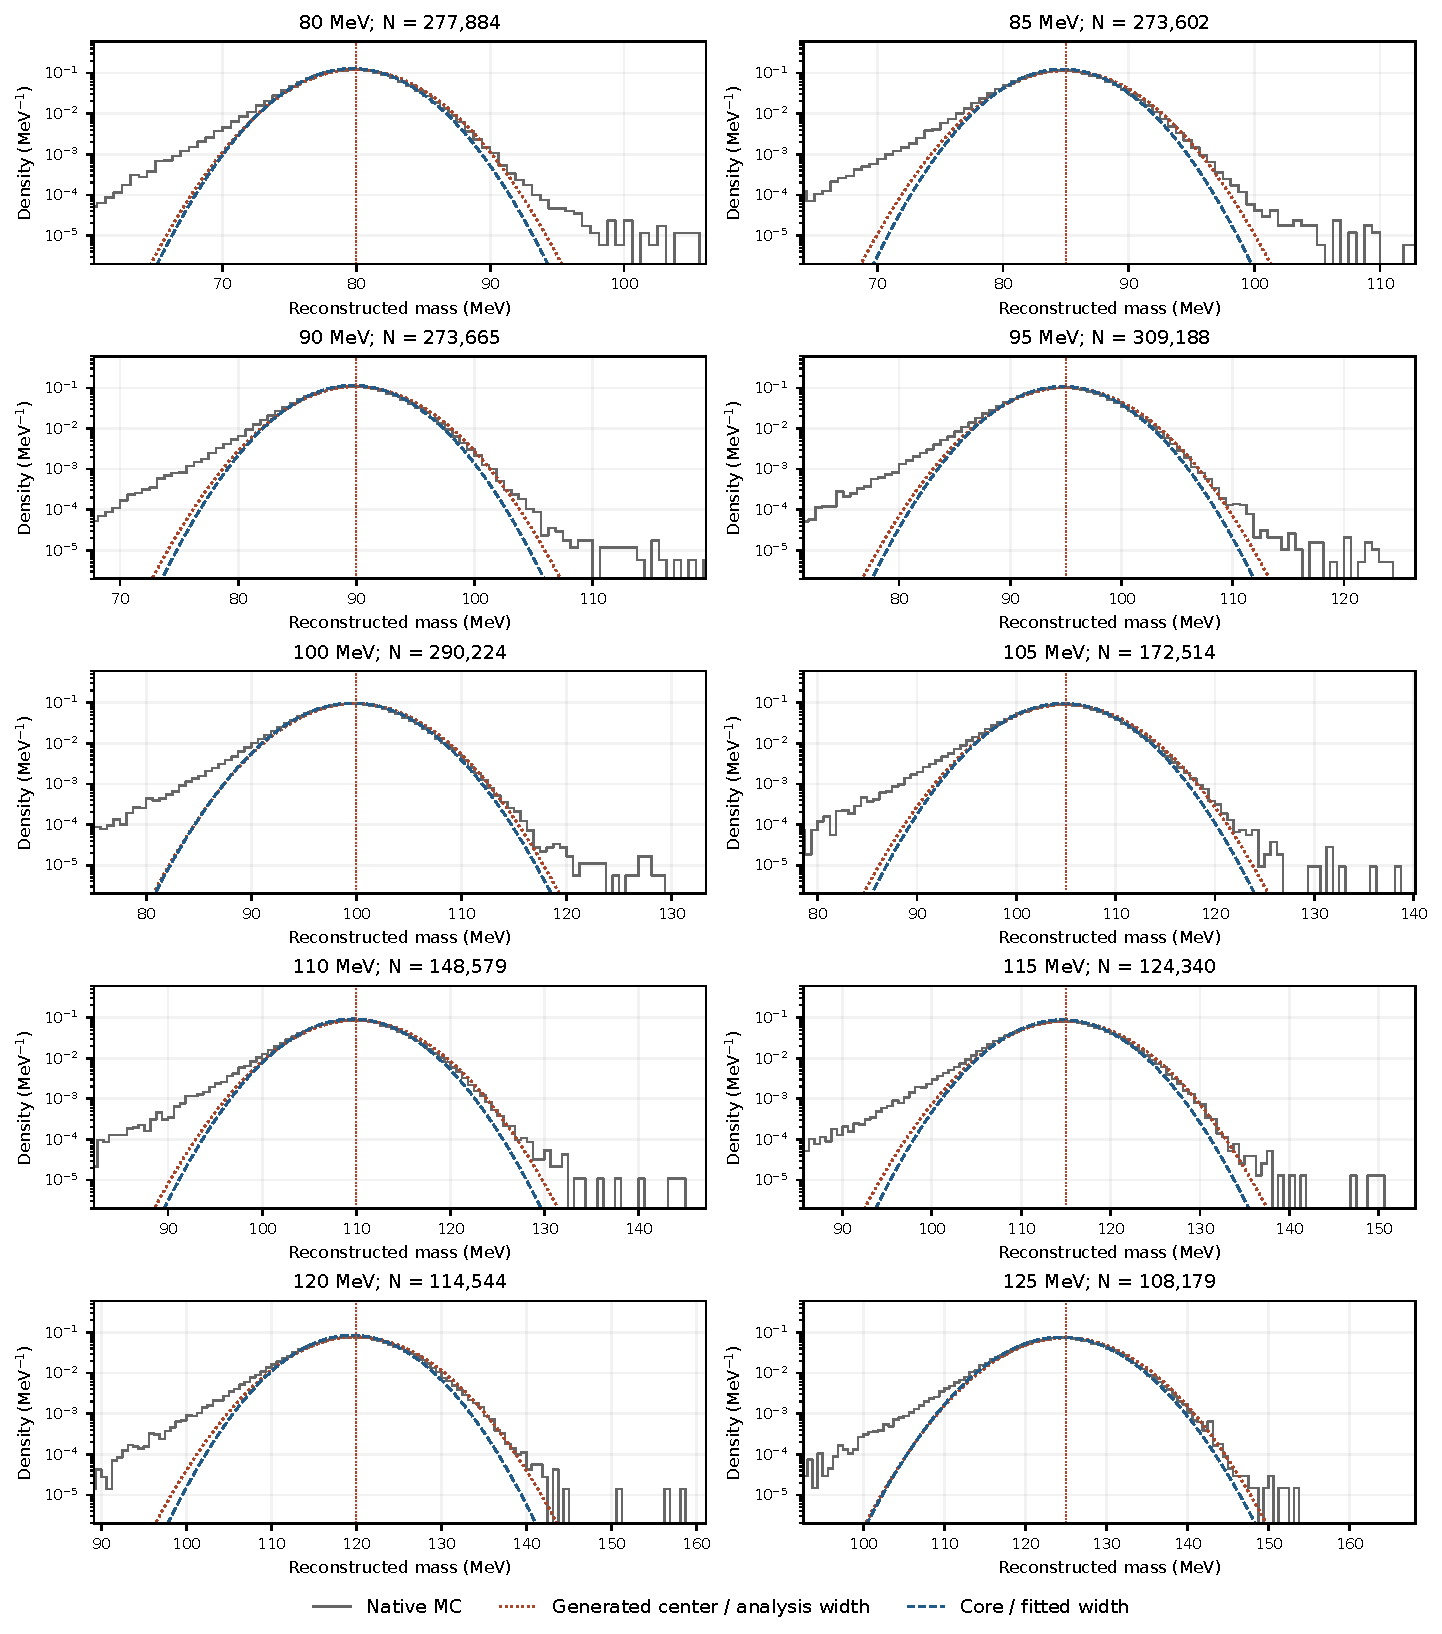
\includegraphics[width=\linewidth,height=6.65in,keepaspectratio]{../figures/shape_catalogue_2.pdf}\end{center}
{\small\refstepcounter{figure}\textbf{Figure \thefigure. How to read the figure.} Gray: native MC. Red dotted: Gaussian at the generated mass with the reference analysis width. Blue dashed: Gaussian at the fitted core with its fitted width. Both Gaussians have unit full area. The logarithmic scale reveals shoulders and tails that are less visible on a linear scale. The empirical MC template used for extraction retains those features; the Gaussians provide visual comparisons.}\par\medskip

\clearpage\section*{Native signal-MC catalogue: 130--175 MeV}
\begin{center}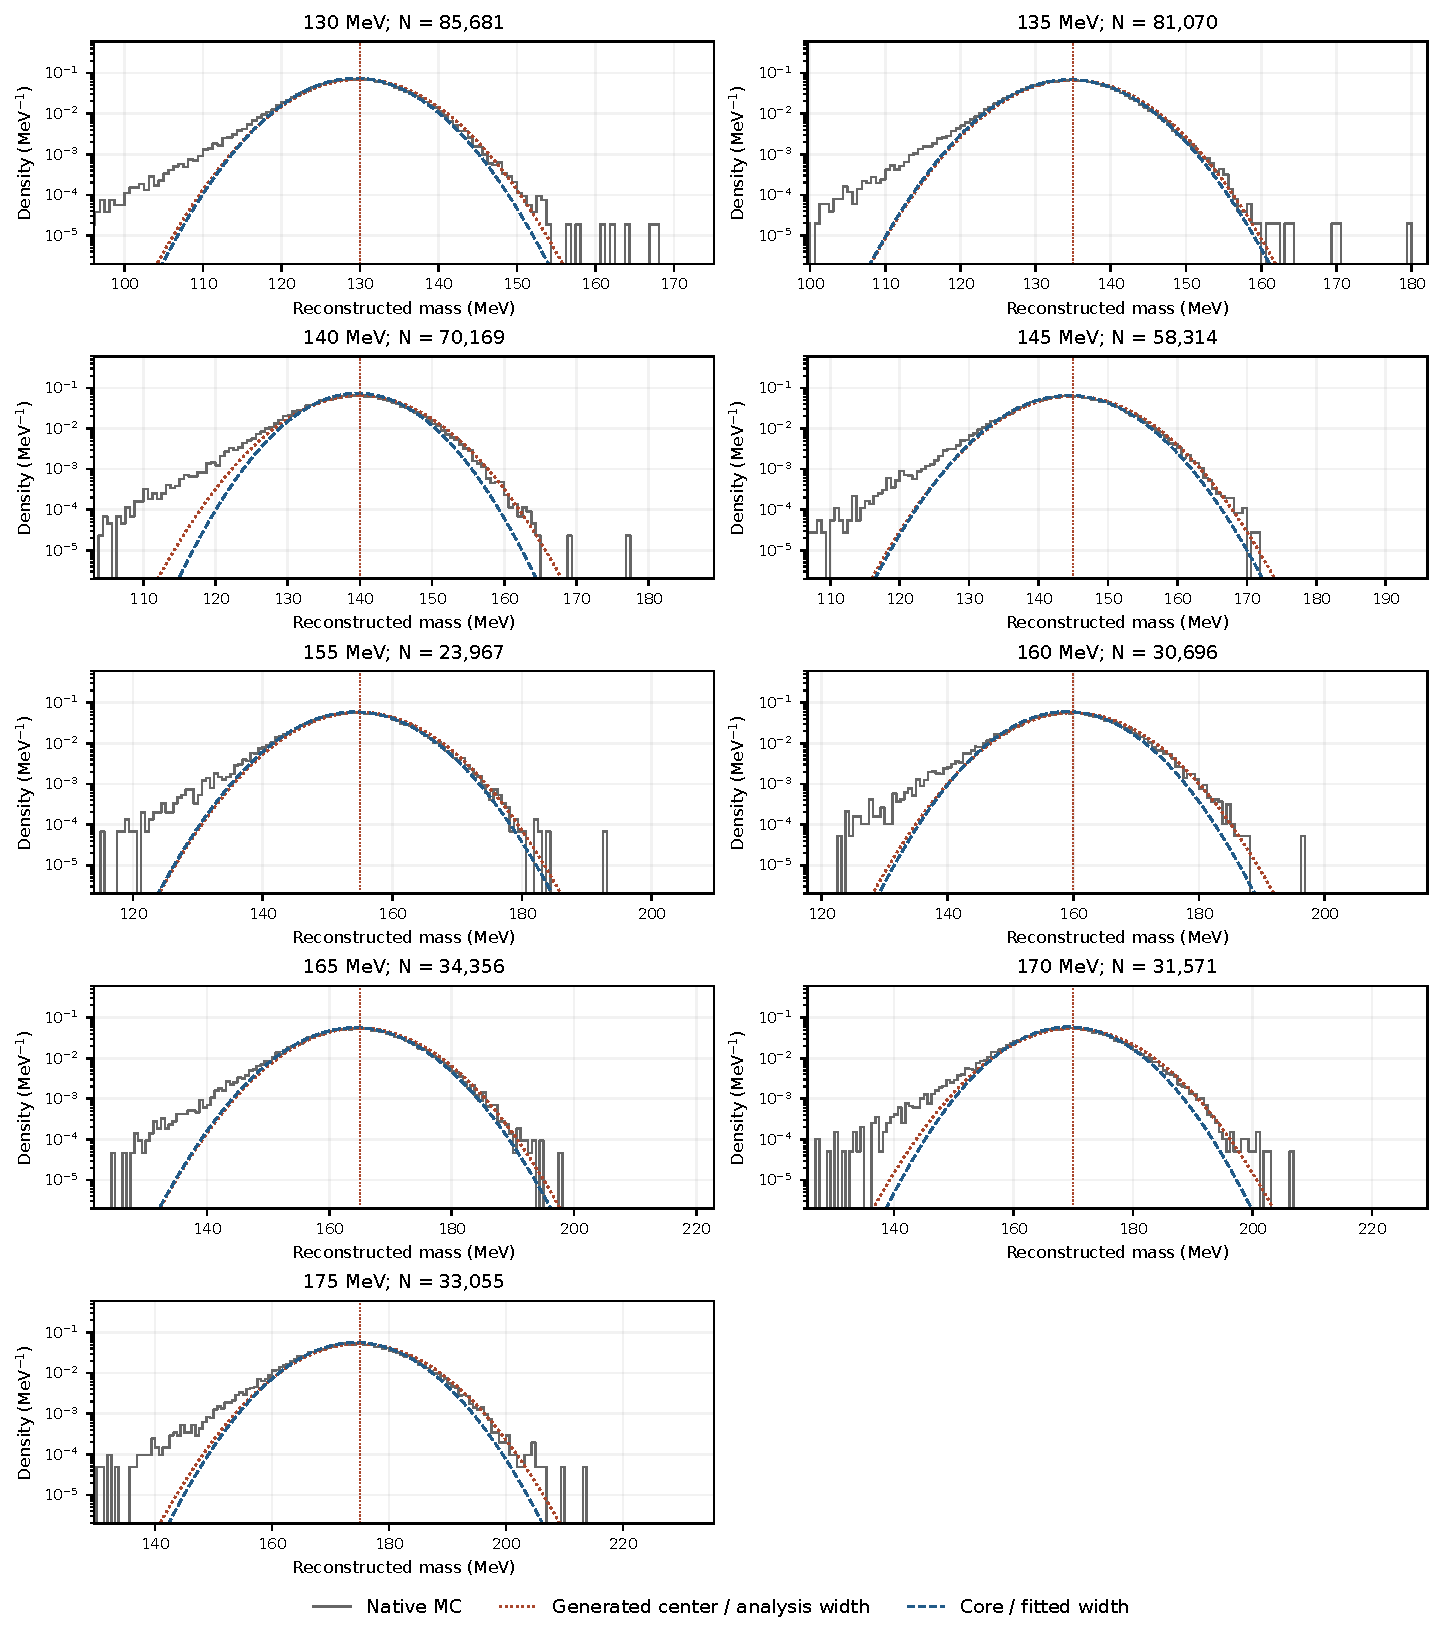
\includegraphics[width=\linewidth,height=6.65in,keepaspectratio]{../figures/shape_catalogue_3.pdf}\end{center}
{\small\refstepcounter{figure}\textbf{Figure \thefigure. How to read the figure.} Gray: native MC. Red dotted: Gaussian at the generated mass with the reference analysis width. Blue dashed: Gaussian at the fitted core with its fitted width. The available inputs jump from 145 to 155 MeV; no simulated 150 MeV histogram is shown. All displayed densities retain their full selected normalization. The high-mass center errors and definition spreads are listed in the preceding table.}\par\medskip
\clearpage\section*{Appendix A. Test a narrower 2016 window: $\pm2u$}
\label{sec:windowappendix}

\textbf{The finding.} Reducing the 2016 MC fit and GP-training exclusion from $\pm3.5u$ to $\pm2u$ lowers most conditional observed profile limits. However, it also reduces the fitted response to an injected full MC signal. In the five tested injections, the narrower window recovers 87.7--92.2\% of the added selected yield, compared with 99.8--100.1\% for the main window. Its smaller raw fit uncertainty therefore does not establish an improvement in signal sensitivity.

\textbf{A controlled window comparison.} Both choices use the same neighboring MC template, $u=(m_{\rm rec}-c)/s$, and the same interpolated core center and width. Only the interval changes. For the comparison, bins with centers satisfying $|u|\le2$ enter the signal likelihood and are excluded from GP training. All other bins enter training. There is no separate extra exclusion. The full selected template normalization, GP kernel settings and inherited coupling conversion are retained; the GP mean and covariance are recomputed for the new sidebands.
\begin{center}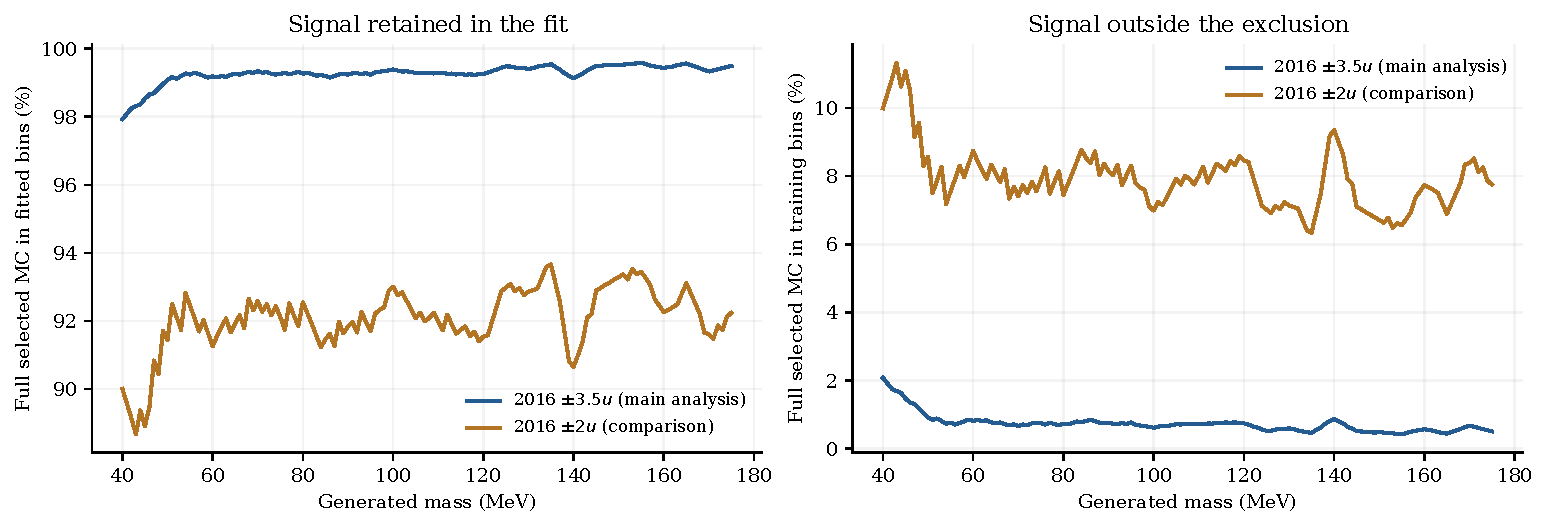
\includegraphics[width=\linewidth,height=2.65in,keepaspectratio]{../figures/window_geometry.pdf}\end{center}
{\small\refstepcounter{figure}\textbf{Figure \thefigure. How to read the figure.} Blue is the main $\pm3.5u$ prescription; gold is $\pm2u$. Left: full selected MC probability in the actual analysis bins used for fitting. Right: probability in the GP-training bins. Bin membership follows bin centers, so the plotted fractions include the finite analysis binning. These are geometric fractions, not detector efficiencies or fitted recovery fractions.}\par\medskip

The narrower fitted bins contain 88.68--93.66\% of the full selected signal over 40--175 MeV, compared with 97.93--99.58\% in the main window. Consequently, 6.34--11.32\% can enter training rather than 0.42--2.07\%. The tail probability is retained in the injections. It is never dropped or renormalized into the fitted interval.

\begin{center}\small\begin{tabular}{rrrrr}\toprule
Mass [MeV] & Window & Actual fit interval [MeV] & Fit bins & MC fraction [\%]\\\midrule
69 & $\pm3.5u$ & 59.50--78.25 & 75 & 99.29\\
69 & $\pm2u$ & 63.50--74.25 & 43 & 92.32\\
91 & $\pm3.5u$ & 78.50--103.00 & 98 & 99.27\\
91 & $\pm2u$ & 83.75--97.75 & 56 & 91.97\\
\bottomrule\end{tabular}\end{center}
The main-body results remain the $\pm3.5u$ analysis. This appendix tests an alternative; it does not replace that prescription.

\clearpage\section*{Appendix A.1. The 2016 observed scan}
The two windows are evaluated at the same 136 hypotheses, 40--175 MeV in 1 MeV steps. Limits continue to refer to the full selected MC yield. The signal shape itself is identical in the two fits.
\begin{center}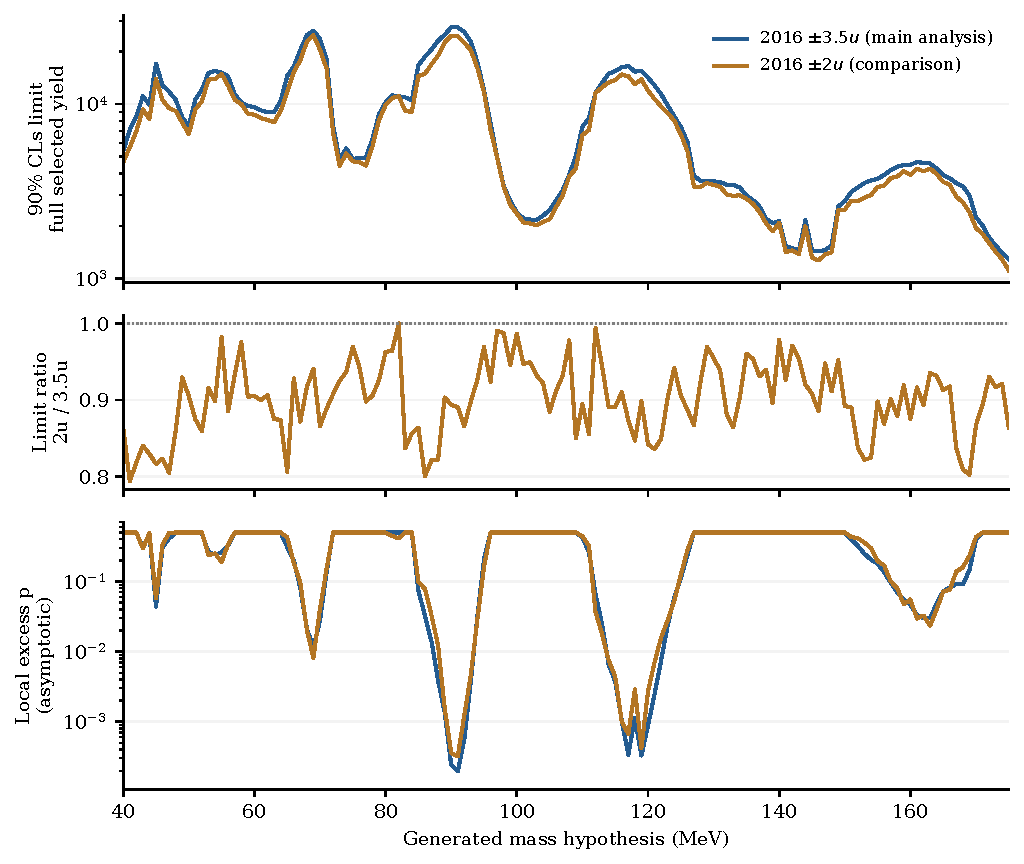
\includegraphics[width=\linewidth,height=4.55in,keepaspectratio]{../figures/window_2016.pdf}\end{center}
{\small\refstepcounter{figure}\textbf{Figure \thefigure. How to read the figure.} Top: conditional observed 90\% profile-$CL_s$ upper limits for the two windows. Middle: the $\pm2u$ limit divided by the $\pm3.5u$ limit at the same mass. Bottom: fixed-mass local asymptotic excess probabilities. These curves use the likelihood and conversion defined in the main text; they are not full-scan toy-calibrated limits or global probabilities.}\par\medskip

The median limit change is $-9.64\%$, with a range of $-20.63\%$ at 41 MeV to $+0.05\%$ at 82 MeV. At 91 MeV, the strongest local feature under both choices, the fitted yield changes from $20{,}201\pm5{,}699$ to $17{,}815\pm5{,}221$ events. The upper limit falls from 27,505 to 24,507 events, while the local asymptotic probability increases from 0.000196 to 0.000321 ($Z=3.55$ to 3.41).

At the other previously selected region, 69 MeV, the fitted yield changes from $16{,}791\pm7{,}371$ to $16{,}115\pm6{,}705$ events, the upper limit from 26,285 to 24,739 events, and the local asymptotic probability from 0.01136 to 0.00812. These fixed-mass comparisons keep the two earlier examples; they do not select a new pair of independent excesses.

\clearpage\section*{Appendix A.2. Propagate only the 2016 window change}
This comparison starts from the final main-body combination: 2015 Gaussian, 2016 neighboring MC and 2021 neighboring MC. The 2021 interval remains $[-4,+3]u$. Campaign availability, observations, full signal probabilities and coupling conversion are identical; only the 2016 fit/exclusion changes.
\begin{center}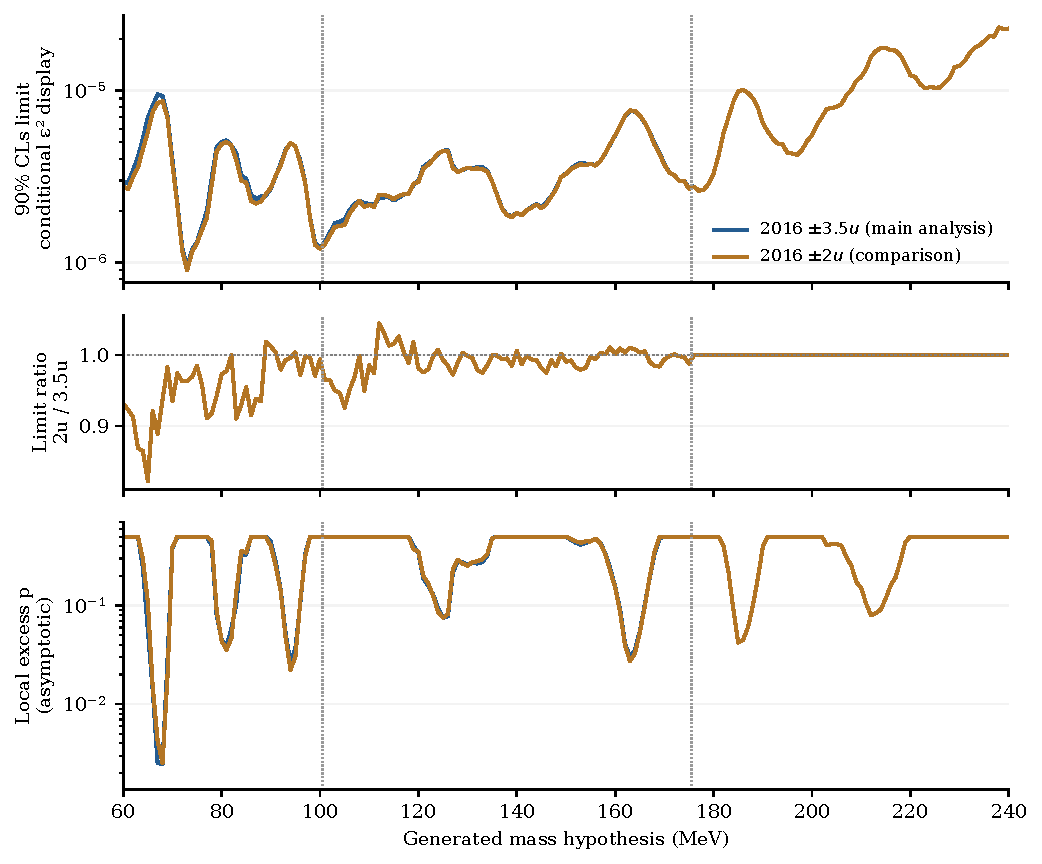
\includegraphics[width=\linewidth,height=4.55in,keepaspectratio]{../figures/window_combined.pdf}\end{center}
{\small\refstepcounter{figure}\textbf{Figure \thefigure. How to read the figure.} Top: the conditional coupling-limit display for the main combination and the combination with 2016 narrowed to $\pm2u$. Middle: their ratio. Bottom: local asymptotic excess probabilities from the joint common-signal likelihood. Vertical dotted lines mark the ends of 2015 and 2016 participation. Above 175 MeV only 2021 contributes, so both curves coincide exactly. No new global probability or efficiency correction is inferred.}\par\medskip

Over 60--175 MeV, where 2016 contributes, the combined upper limit changes by a median $-1.36\%$. The range is $-17.83\%$ at 65 MeV to $+4.49\%$ at 112 MeV. The effect is smaller than the typical 2016-only shift because the common signal parameter must also describe the other included campaigns.

The strongest combined local feature stays at 68 MeV: $p_0$ changes only from 0.002475 to 0.002539 ($Z=2.810$ to 2.802). The narrower-window scan remains a conditional profile comparison. The main-body selected-point rank calibration used the wider 2016 prescription and is not transferred to this alternative.

\clearpage\section*{Appendix A.3. Does the narrower window recover the signal?}

At 60, 69, 91, 100 and 160 MeV, 200 paired experiments add the same full MC signal to the same fixed GP-mean background for both windows. The expected selected yield is $A=3s_0$, where $s_0$ is the wider-window MC fit's Hessian error on the fixed background mean. Each stored-bin and outside-support signal category is Poisson sampled. Background-only and signal-injected fits share their background draw; neither the observed spectrum nor a fitted null bias determines the injected yield.

The response below is $R=\langle\Ah_{s+b}-\Ah_b\rangle/A$. Pairing removes the background-only mean from this response measurement; no correction is applied to the observed fits.
\begin{center}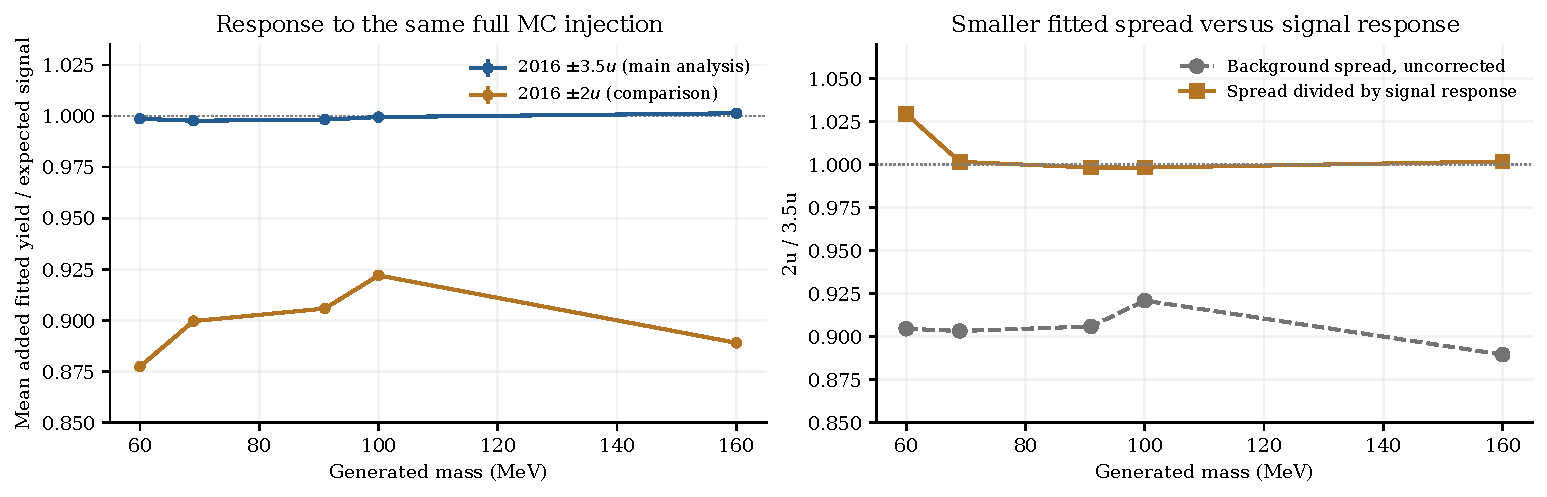
\includegraphics[width=\linewidth,height=2.65in,keepaspectratio]{../figures/window_response.pdf}\end{center}
{\small\refstepcounter{figure}\textbf{Figure \thefigure. How to read the figure.} Left: response to the same expected full selected signal; error bars are Monte Carlo standard errors of the paired mean. Right: the ratio of background-toy fitted-yield spreads, before and after dividing each spread by its response. The ratios are descriptive point estimates from 200 paired experiments; their few-percent differences are not precise sensitivity improvements. Neither panel measures coverage.}\par\medskip

The narrower response is 0.877--0.922, while the wider response is 0.998--1.001. Dividing the background fitted-yield spread by the response gives narrow/wide ratios of 0.998--1.030. Thus the smaller raw fitted spread is largely offset by the reduced response. Together with the extra signal in training bins, this is consistent with increased signal absorption by the background estimate. It supports retaining $\pm3.5u$ as the main choice in this bounded comparison.

\textbf{Local background check.} Both windows also use the same 1,000 fixed-source null draws at 69 and 91 MeV. At 91 MeV, $\pm2u$ has 1 exceedance, rank $2/1001=0.0020$, and a 95\% exact binomial interval [0.000025, 0.00556]; $\pm3.5u$ has 3, rank 0.0040, with [0.00062, 0.00874]. At 69 MeV the counts are 3 and 5, with ranks 0.0040 and 0.0060 and intervals [0.00062, 0.00874] and [0.00163, 0.01163]. These sparse, paired tails do not establish a significant difference between windows. The positive mean null root at 91 MeV remains: 0.601 versus 0.656.

\textbf{Record and scope.} The appendix adds 252 observed fits and 6,000 toy fits, reusing 2,000 matching main-body null rows. Complete signed yields, Hessian errors, pulls, realized signal partitions, pairing hashes and probability intervals are under \path{results/window_comparison}. This is a five-mass, one-strength, fixed-source response check, not an independent coverage validation or a new calibrated upper-limit construction. Rebuild the appendix with \path{rebuild_appendix.sh}; the parent numerical records remain unchanged.
\end{document}
